\documentclass[aspectratio=169]{beamer}
%
% Choose how your presentation looks.
%
% For more themes, color themes and font themes, see:
% http://deic.uab.es/~iblanes/beamer_gallery/index_by_theme.html
%
\mode<presentation>
{
  \usetheme{metropolis}      % or try Darmstadt, Madrid, Warsaw, ...
  \usecolortheme{metropolis-imagelab} % or try albatross, beaver, crane, ...
  \usefonttheme{structurebold}  % or try serif, structurebold, ...
  \setbeamercolor{background canvas}{bg=white}
  \setbeamertemplate{navigation symbols}{}
  \setbeamertemplate{bibliography item}{\insertbiblabel}
  %\setbeamertemplate{caption}[numbered]
} 
\usepackage[english]{babel}
\usepackage[utf8x]{inputenc}
\usepackage{hyperref}
\usepackage{algorithm,algorithmic}
\usepackage{listings}             % Include the listings-package
\usepackage{pgfplots}
\usepackage{caption}
\usepackage{xcolor}
\usepackage{amsmath}

\usepackage{tikz}
\usepackage{animate}
\usepackage{bm}


\hypersetup{
    colorlinks = true,
    linkcolor = {black},
    urlcolor = {mImagelabRed}
}

\DeclareMathOperator*{\argmin}{arg\,min}
\DeclareMathOperator*{\argmax}{arg\,max}
\newcommand{\highlight}[1]{\textcolor{mImagelabRed}{#1}}

\title[Reinforcement Learning]{Reinforcement Learning}
\subtitle{Introduction and Model-Free Learning}
\institute{University of Modena and Reggio Emilia}
\author{Davide Abati}
\date{\today}

\def\thisframelogos{}

\newcommand{\framelogo}[1]{\def\thisframelogos{#1}}
%\algnewcommand{\myRepeat}[1]{\State \algorithmicrepeat \unskip #1}

\begin{document}

\framelogo{logo_unimore_white.png}

\bgroup
\renewcommand{\insertframenumber}{}
\begin{frame}[noframenumbering]
  \titlepage
\end{frame}
\egroup
\bgroup
\begin{frame}{Disclaimer}
All this material is a free re-arrangement of \href{http://www0.cs.ucl.ac.uk/staff/d.silver/web/Teaching.html}{David Silver's UCL Course on RL}.
\\
You are also encouraged to take a look to his \href{https://www.youtube.com/watch?v=2pWv7GOvuf0}{Youtube lectures}.
\end{frame}
\egroup

\section{What is reinforcement learning?}
\bgroup
\begin{frame}{Branches of Machine Learning}
\begin{figure}
\centering
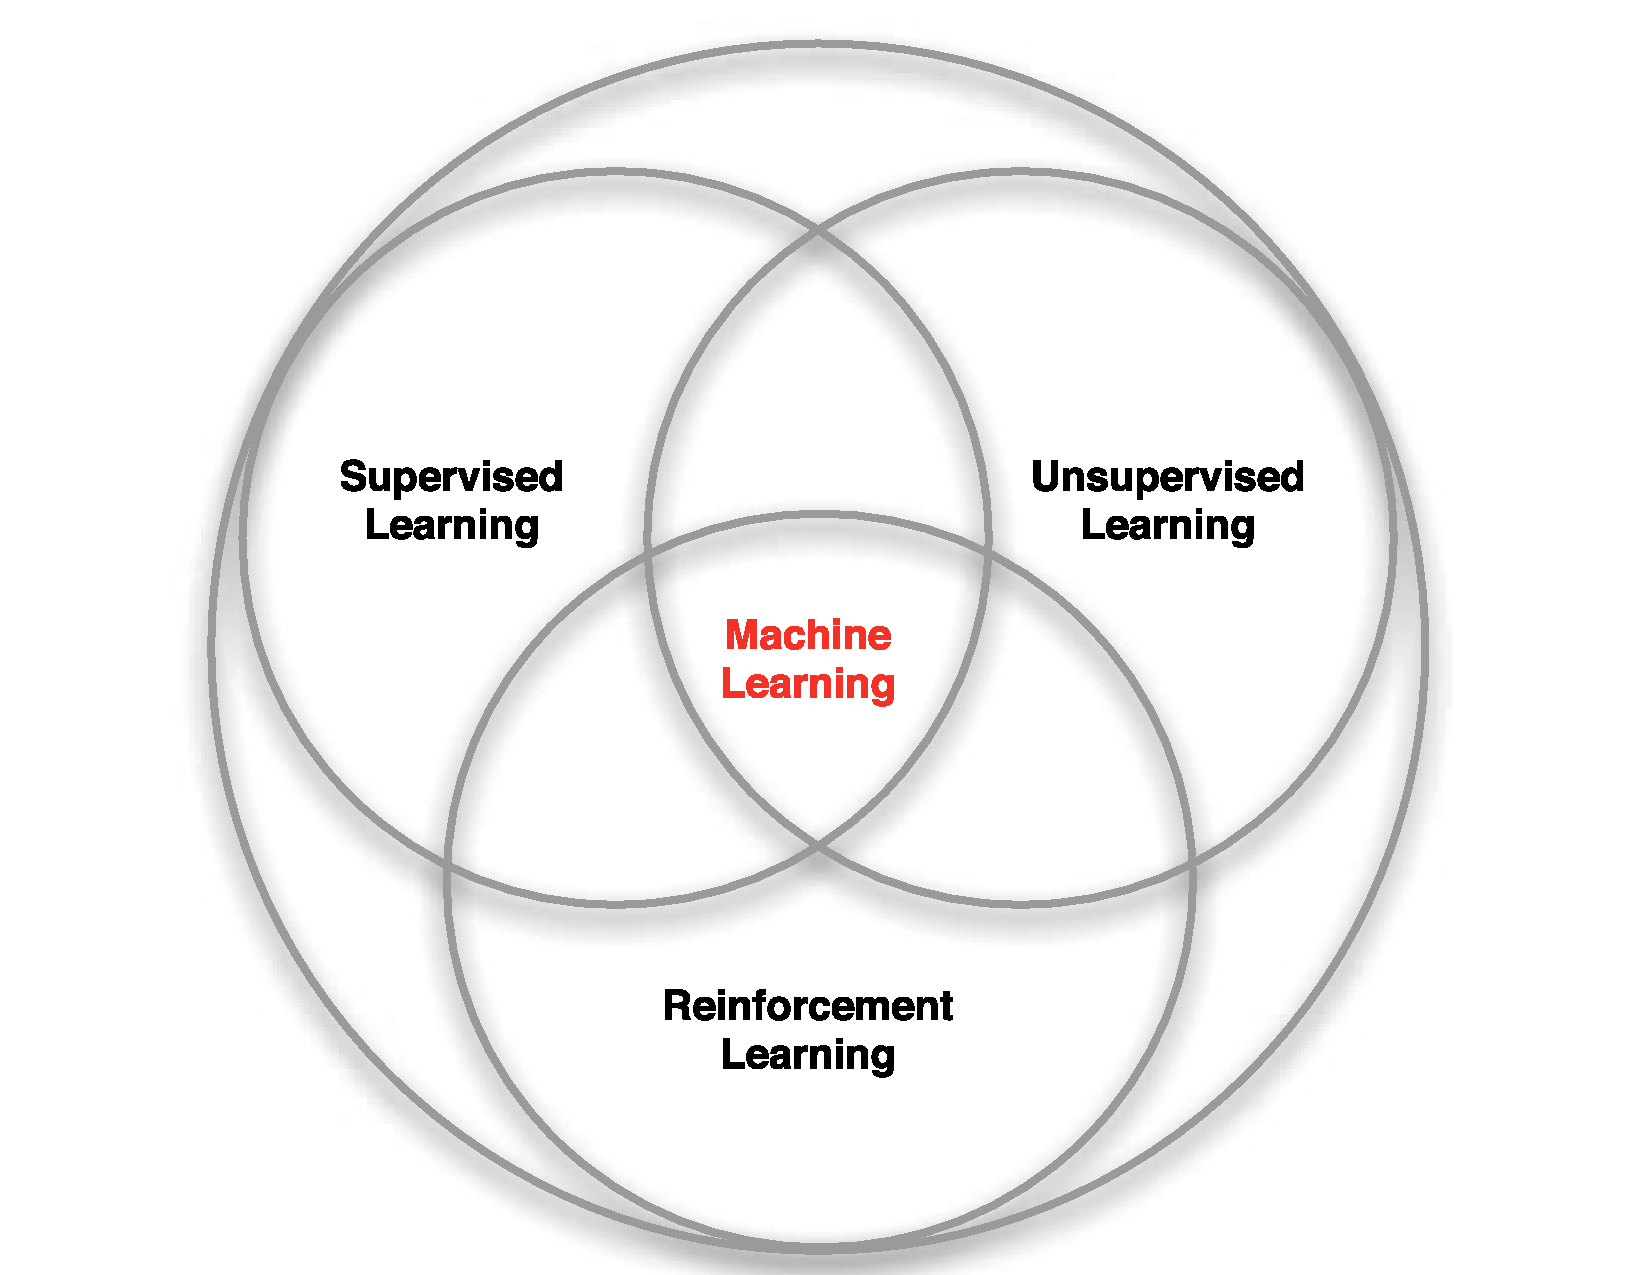
\includegraphics[width=0.6\textwidth]{img/ml_taxonomy.pdf}
\end{figure}
\end{frame}
\egroup
\bgroup
\begin{frame}{RL Characteristics}
What makes reinforcement learning different from other machine learning paradigms?
\begin{itemize}
\item There is no supervisor, only a \emph{reward} signal.
\item Feedback is delayed, not instantaneous
\item Time really matters (sequential, non i.i.d. data)
\item Agent is \emph{active}: its actions affect the environment he lives in.
\end{itemize}
\end{frame}
\egroup
\bgroup
\begin{frame}{Rewards}
\begin{itemize}
\item A \highlight{reward} $R_t$ is a scalar feedback signal
\item Indicates how well agent is doing at step $t$
\item The agent's job is to maximise cumulative reward over an episode
\end{itemize}
\end{frame}
\egroup
\bgroup
\begin{frame}{Rewards: examples}
\begin{itemize}
\item Fly stunt manoeuvres in a helicopter
\begin{itemize}
\item +ve reward for following desired trajectory
\item -ve reward for crashing
\end{itemize}
\item Defeat the world champion at Go
\begin{itemize}
\item +ve/-ve reward for winning/losing a game
\end{itemize}
\item Make a humanoid robot walk
\begin{itemize}
\item +ve reward for forward motion
\item -ve reward for falling over
\end{itemize}
\item Play Atari games better than humans
\begin{itemize}
\item +ve reward for increasing/decreasing score
\end{itemize}
\end{itemize}
\end{frame}
\egroup

\section{Inside a RL agent}
\bgroup
\begin{frame}{Sequential Decision Making}
\begin{itemize}
\item Goal: \emph{select actions to maximise total future reward}
\item Actions may have long term consequences
\item Reward may be delayed
\item It may be better to sacrifice immediate reward to gain more long-term reward.
\begin{itemize}
\item A financial investment may take months to mature
\item Refuelling a helicopter now might prevent a crash in several hours
\item Blocking opponent moves might help winning chances many moves from now
\end{itemize}
\end{itemize}
\end{frame}
\egroup
\bgroup
\begin{frame}{Agent and environment}
\begin{minipage}{0.45\textwidth}
\begin{figure}
\centering
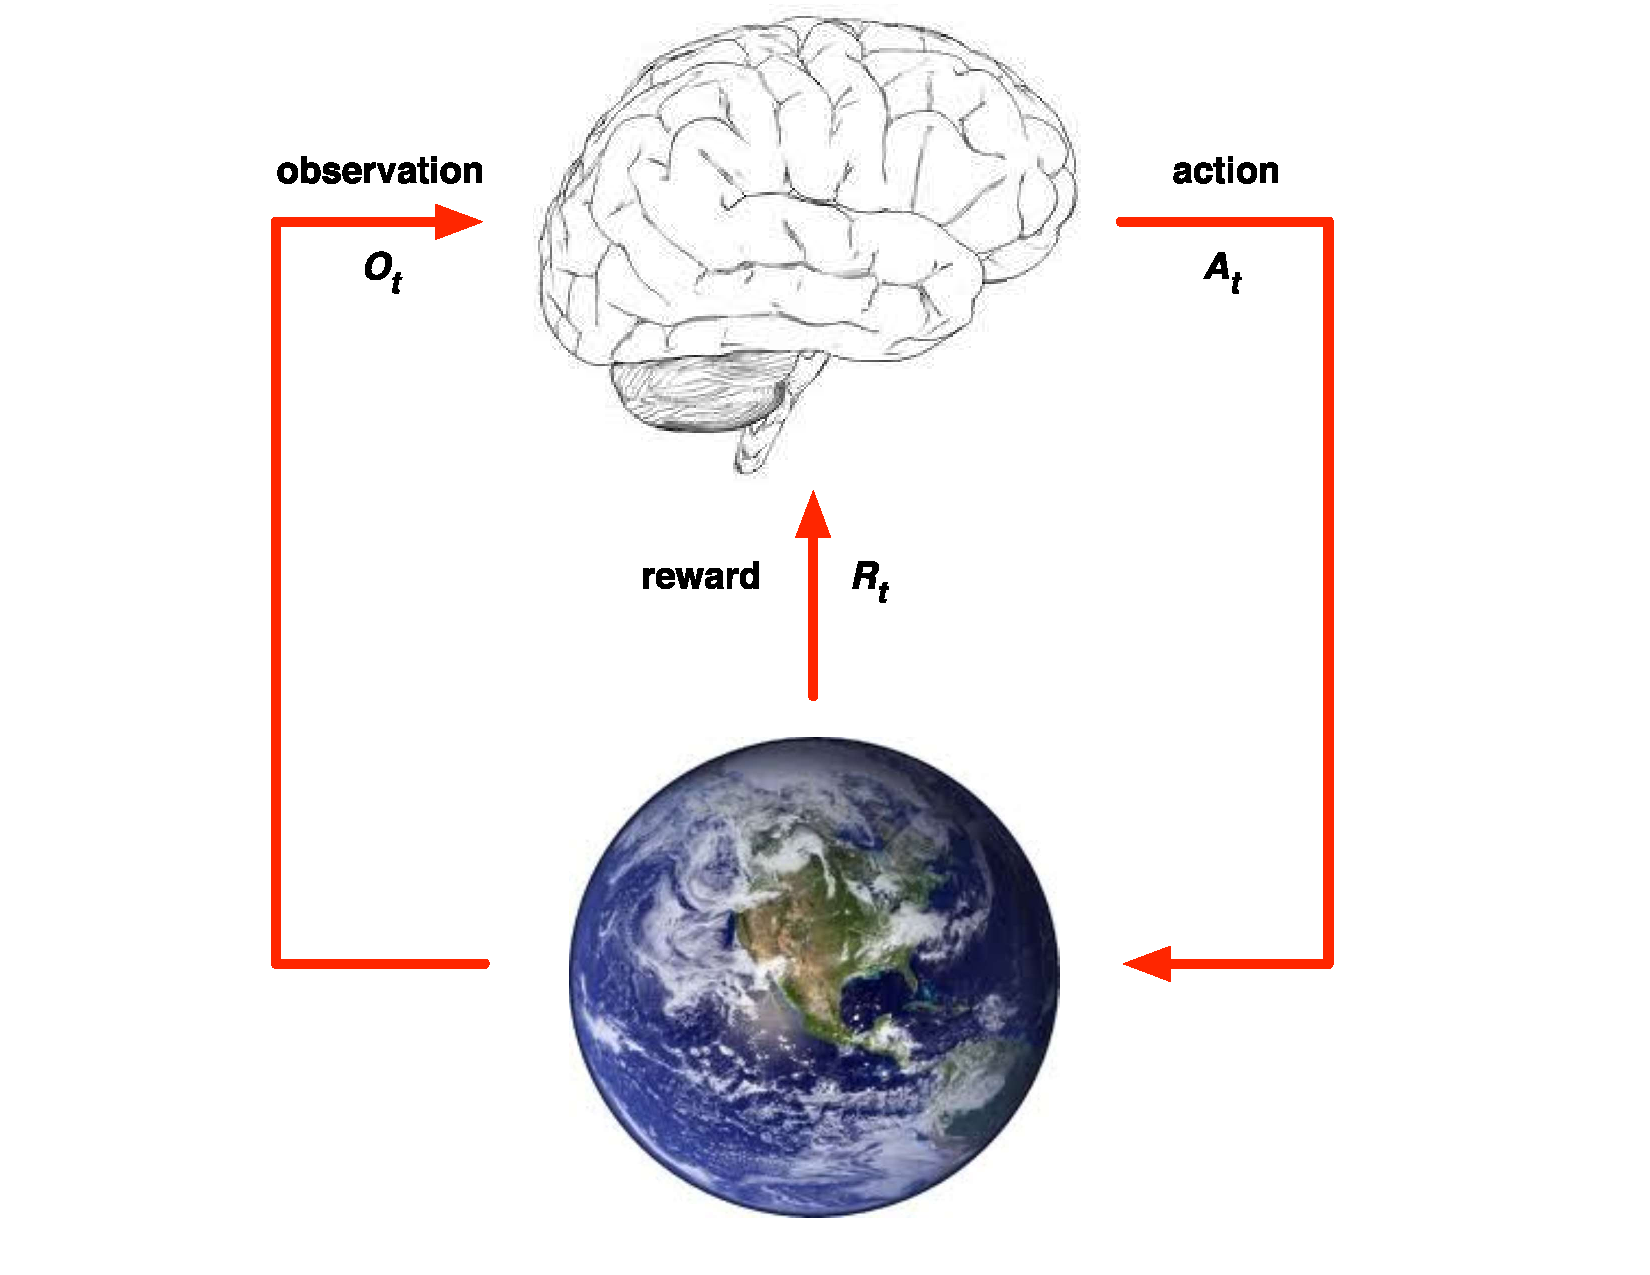
\includegraphics[width=\textwidth]{img/agent_and_environment.pdf}
\end{figure}
\end{minipage}
\begin{minipage}{0.45\textwidth}
\begin{itemize}
\item At each step $t$ the agent:
\begin{itemize}
\item Receives observation $O_t$
\item Receives scalar reward $R_t$
\item Executes action $A_t$
\end{itemize}
\item The environment:
\begin{itemize}
\item Receives action $A_t$
\item Emits observation $O_{t+1}$
\item Emits scalar reward $R_{t+1}$
\end{itemize}
\item $t$ increments at env. step
\end{itemize}
\end{minipage}
\end{frame}
\egroup
\bgroup
\begin{frame}{State}
\begin{itemize}
\item The \highlight{history} is the sequence of observations, actions, rewards
\begin{equation*}
H_t = O_1, R_1, A_1, \ldots, A_{t-1}, O_t, R_t
\end{equation*}
\item The \highlight{state} is the information used to determine what happens next.
\begin{itemize}
\item It is a function of the history:
\begin{equation*}
S_t = f(H_t)
\end{equation*}
\end{itemize}
\end{itemize}
\end{frame}
\egroup
\bgroup
{\renewcommand{\arraystretch}{2} 
\begin{frame}{Agent and environment states}
\centering
\begin{tabular}{l|l}
\multicolumn{1}{c|}{Agent state $S_t^a$}&
\multicolumn{1}{c}{Environment state $S_t^e$}\\
\multicolumn{1}{p{6cm}|}{whatever information the agent uses to pick the next action}&
\multicolumn{1}{p{6cm}}{whatever data the environment uses to pick the next observation/reward}\\
\multicolumn{1}{p{6cm}|}{it is the information used by RL algorithms}&
\multicolumn{1}{p{6cm}}{usually not visible by the agent}
\end{tabular}
\begin{itemize}
\item \highlight{Full observability}: agent directly observes environment state
\item \highlight{Partial observability}: agent indirectly observes environment state
\end{itemize}
\end{frame}
\egroup
\bgroup
\begin{frame}{Inside  a reinforcement learning agent}
\begin{itemize}
\item An agent may include one or more of these components:
\begin{itemize}
\item Policy: agent's behaviour function
\item Value function: how good is each state and/or action
\item Model: representation of the environment
\end{itemize}
\end{itemize}
\end{frame}
\egroup
\bgroup
\begin{frame}{Policy}
\begin{itemize}
\item A \highlight{policy} is the agent's behaviour
\item It is a map from state to action
\item Deterministic policy: $a = \pi(s)$
\item Stochastic policy: $\pi(a|s) = \mathbb{P}[A_t=s | S_t=s]$
\end{itemize}
\end{frame}
\egroup
\bgroup
\begin{frame}{Return}
\begin{block}{Definition}
The return $G_t$ is the total discounted reward from time-step $t$.
\begin{equation*}
G_t = R_{t+1} + \gamma R_{t+2} + \ldots = \sum_{k=0}^{\infty} \gamma^{k}R_{t+k+1}
\end{equation*}
\end{block}
\begin{itemize}
\item The discount $\gamma \in [0, 1]$ is the present value of future rewards
\item The value of receiving reward $R$ after $k + 1$ time-steps is $\gamma^{k} R$.
\item This values immediate reward above delayed reward.
\item $\gamma$ close to 0 leads to \emph{myopic} evaluation
\item $\gamma$ close to 1 leads to \emph{far-sighted} evaluation
\end{itemize}
\end{frame}
\egroup
\bgroup
\begin{frame}{Value function}
\begin{itemize}
\item Value function is a prediction of future reward
\item Used to evaluate goodness/badness of states
\item And therefore to select between actions
\begin{block}{Definition}
The \emph{state-value function} $v_{\pi}(s)$ is the expected return starting from state $s$, and then following policy $\pi$
\begin{equation*}
v_{\pi}(s) = \mathbb{E}_{\pi}[G_t | S_t = s]
\end{equation*}
\end{block}
%
\begin{block}{Definition}
The \emph{action-value function} $q_{\pi}(s, a)$ is the expected return starting from state $s$, taking action $a$, and then following policy $\pi$
\begin{equation*}
q_{\pi}(s, a) = \mathbb{E}_{\pi}[G_t | S_t = s, A_t = a]
\end{equation*}
\end{block}
\end{itemize}
\end{frame}
\egroup
\bgroup
\begin{frame}{Bellman expectation equation}
The value function can be decomposed into two parts:
\begin{itemize}
\item immediate reward $R_{t+1}$
\item discounted value of successor state $\gamma v(S_{t+1})$
\end{itemize}
\begin{align*}
v_{\pi}(s) &= \mathbb{E}_{\pi}[G_t | S_t = s]\\
&= \mathbb{E}_{\pi} [R_{t+1} + \gamma R_{t+2} + \gamma^2 R_{t+3} + \ldots | S_t = s]\\
&= \mathbb{E}_{\pi}[R_{t+1} + \gamma(R_{t+2} + \gamma R_{t+3} + \ldots )| S_t = s]\\
&= \mathbb{E}_{\pi}[R_{t+1} + \gamma G_{t+1} | S_t = s]\\
&= \mathbb{E}_{\pi}[R_{t+1} + \gamma v_{\pi}(S_{t+1}) | S_t = s]
\end{align*}
\end{frame}
\egroup
\bgroup
\begin{frame}{Bellman Expectation Equation}
The state-value function can again be decomposed into immediate reward plus discounted value of successor state,
\begin{equation*}
v_{\pi}(s) = \mathbb{E}_{\pi}[R_{t+1} + \gamma v_{\pi}(S_{t+1}) | S_t = s]
\end{equation*}
The action-value function can similarly be decomposed,
\begin{equation*}
q_{\pi}(s, a) = \mathbb{E}_{\pi}[R_{t+1} + \gamma q_{\pi}(S_{t+1}, A_{t+1}) | S_t = s, A_t = a]
\end{equation*}
\end{frame}
\egroup
\bgroup
\begin{frame}{Model}
\begin{itemize}
\item A \highlight{model} predicts what the environment will do next
\item $\mathcal{P}$ predicts the next state
\item $\mathcal{R}$ predicts the next (immediate) reward
\end{itemize}
\begin{equation*}
\mathcal{P}^a{ss'}=\mathbb{P}[S_{t+1}=s'| S_t=s, A_t=a]
\end{equation*}
\begin{equation*}
\mathcal{R}^a_s = \mathbb{E}[R_{t+1}|S_t=s, A_t=a]
\end{equation*}
\end{frame}
\egroup
\bgroup
\begin{frame}{Maze example}
\begin{minipage}{0.45\textwidth}
\begin{figure}
\centering
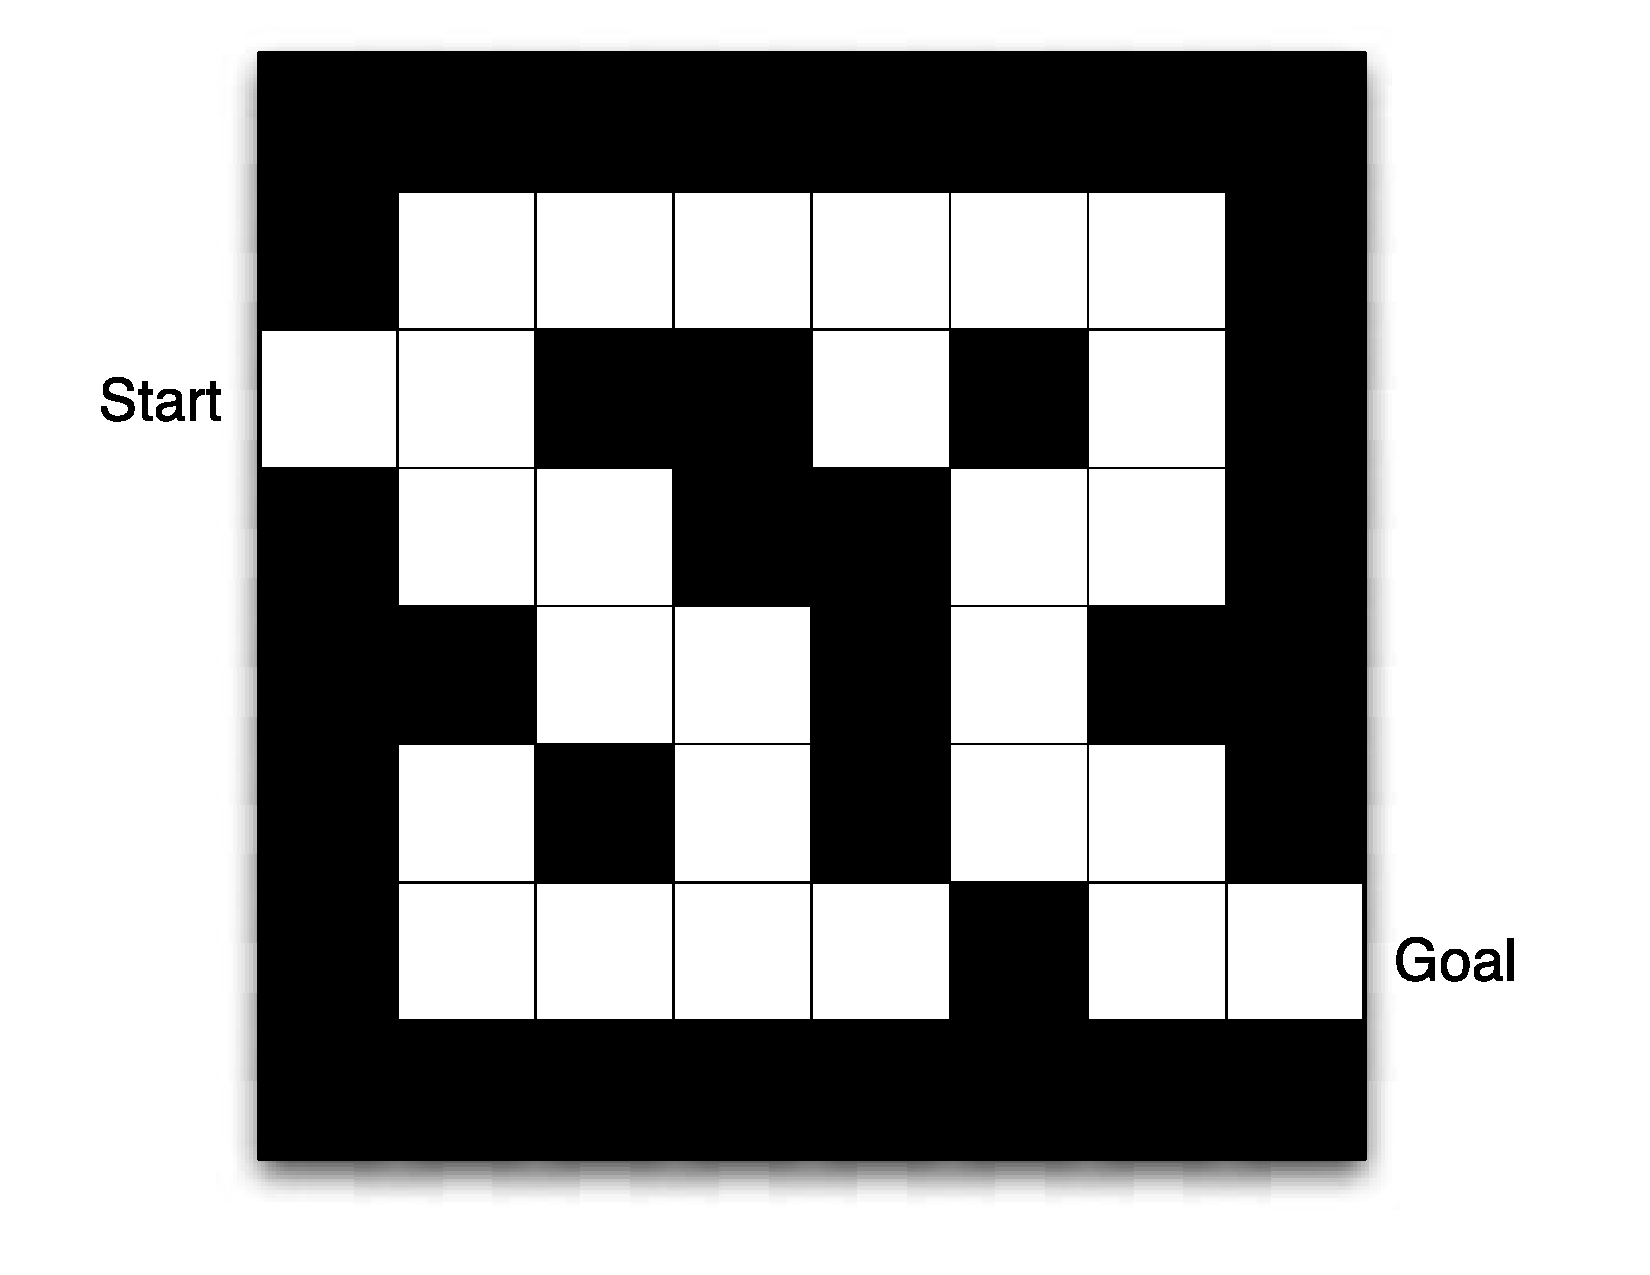
\includegraphics[width=\textwidth]{img/maze_setup.pdf}
\end{figure}
\end{minipage}
\begin{minipage}{0.45\textwidth}
\begin{itemize}
\item Rewards: -1 per time-step
\item Actions: N, S, W, E
\item States: Agent's location
\end{itemize}
\end{minipage}
\end{frame}
\egroup
\bgroup
\begin{frame}{Maze example: policy}
\begin{figure}
\centering
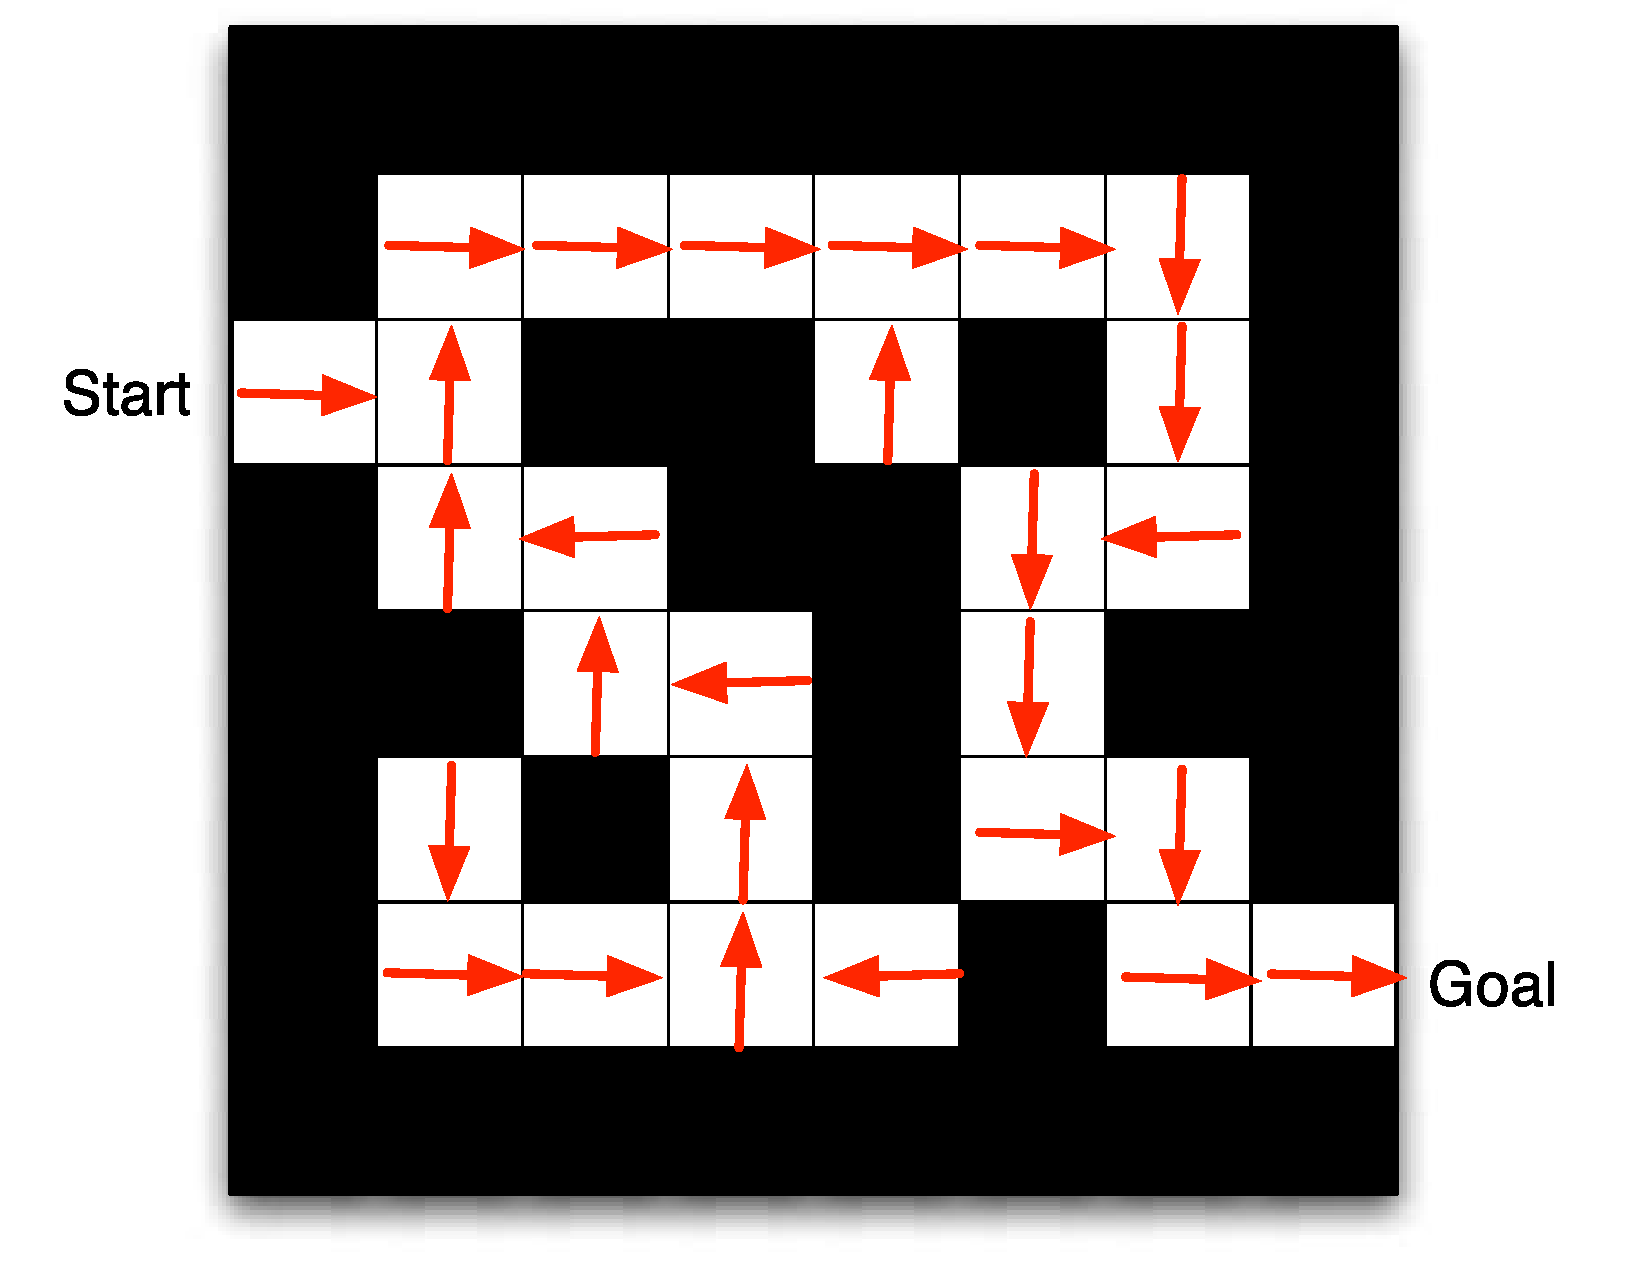
\includegraphics[width=0.5\textwidth]{img/maze_policy.pdf}
\end{figure}
\begin{itemize}
\item Arrows represent policy $\pi(s)$ for each state $s$
\end{itemize}
\end{frame}
\egroup
\bgroup
\begin{frame}{Maze example: value function}
\begin{figure}
\centering
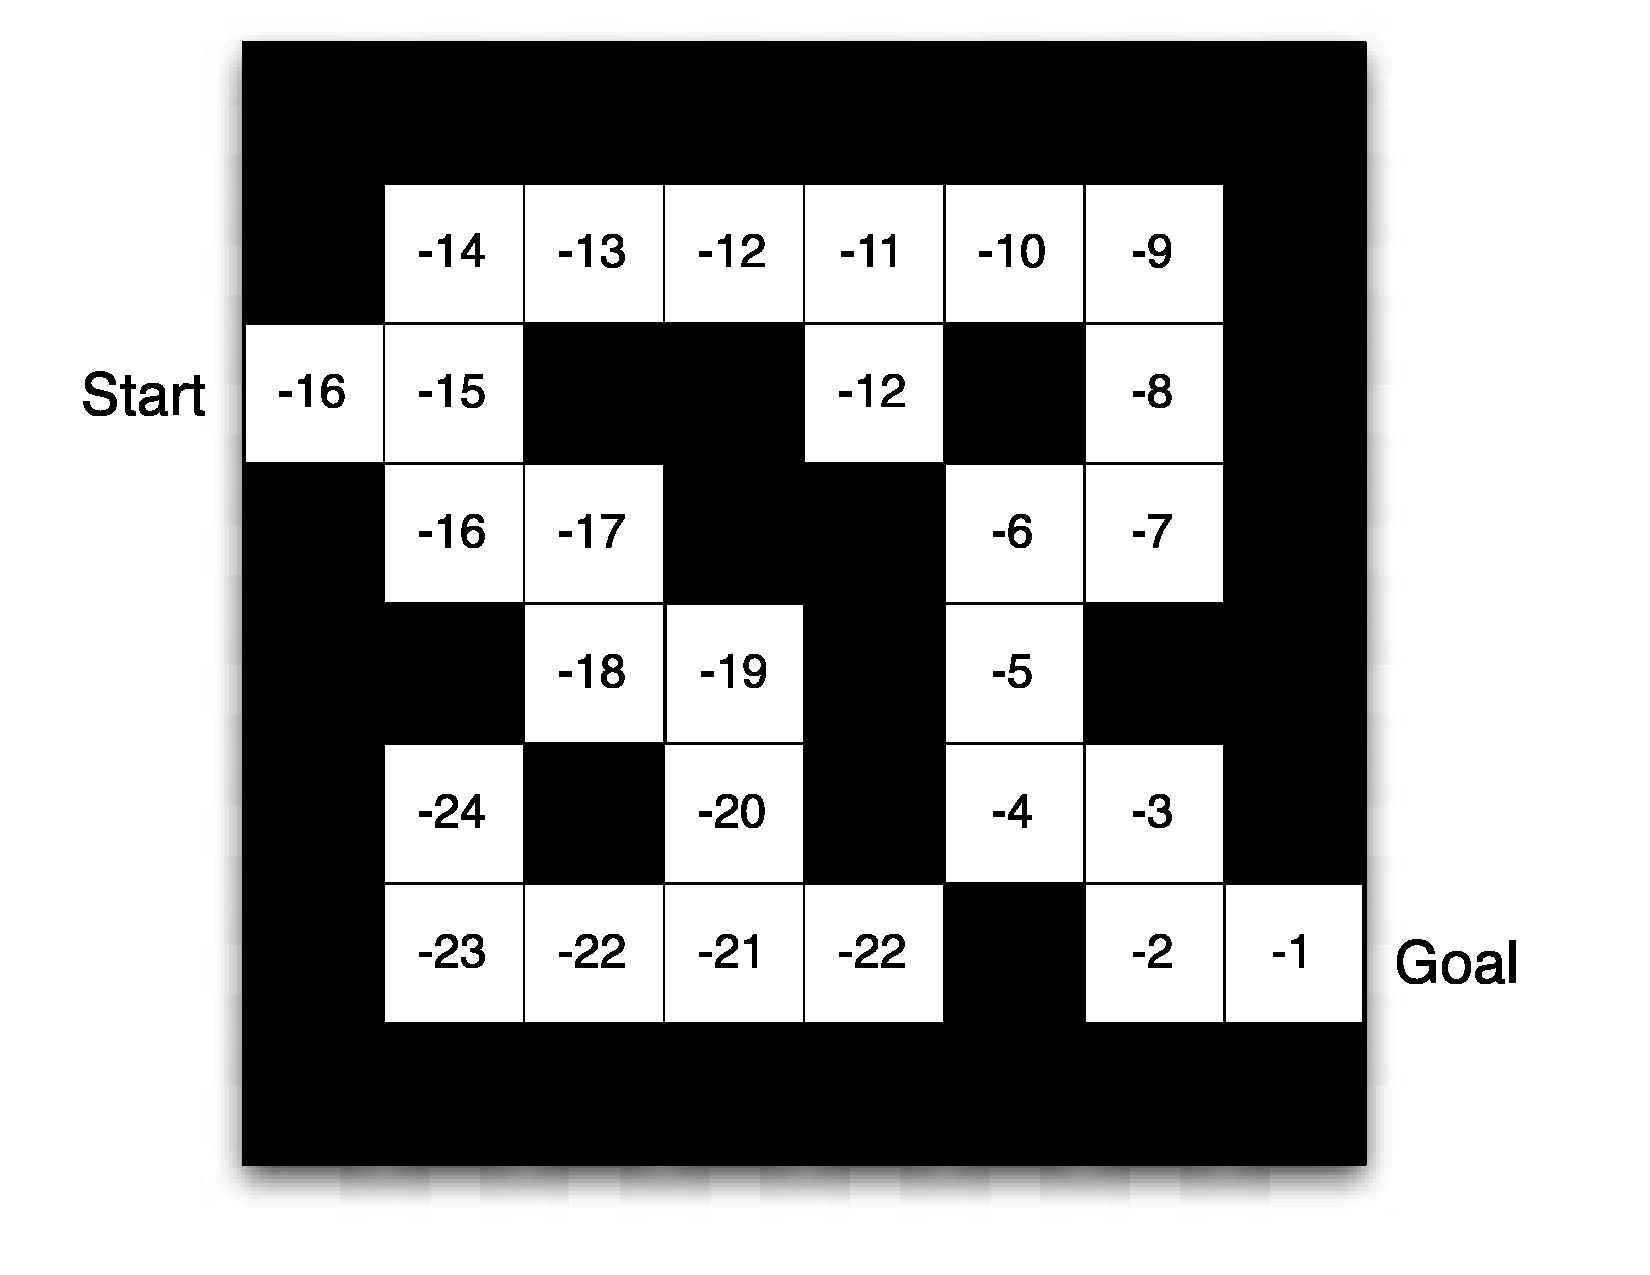
\includegraphics[width=0.5\textwidth]{img/maze_value.pdf}
\end{figure}
\begin{itemize}
\item Numbers represent policy $v_{\pi}(s)$ for each state $s$
\end{itemize}
\end{frame}
\egroup
\bgroup
\begin{frame}{Maze example: model}
\begin{figure}
\centering
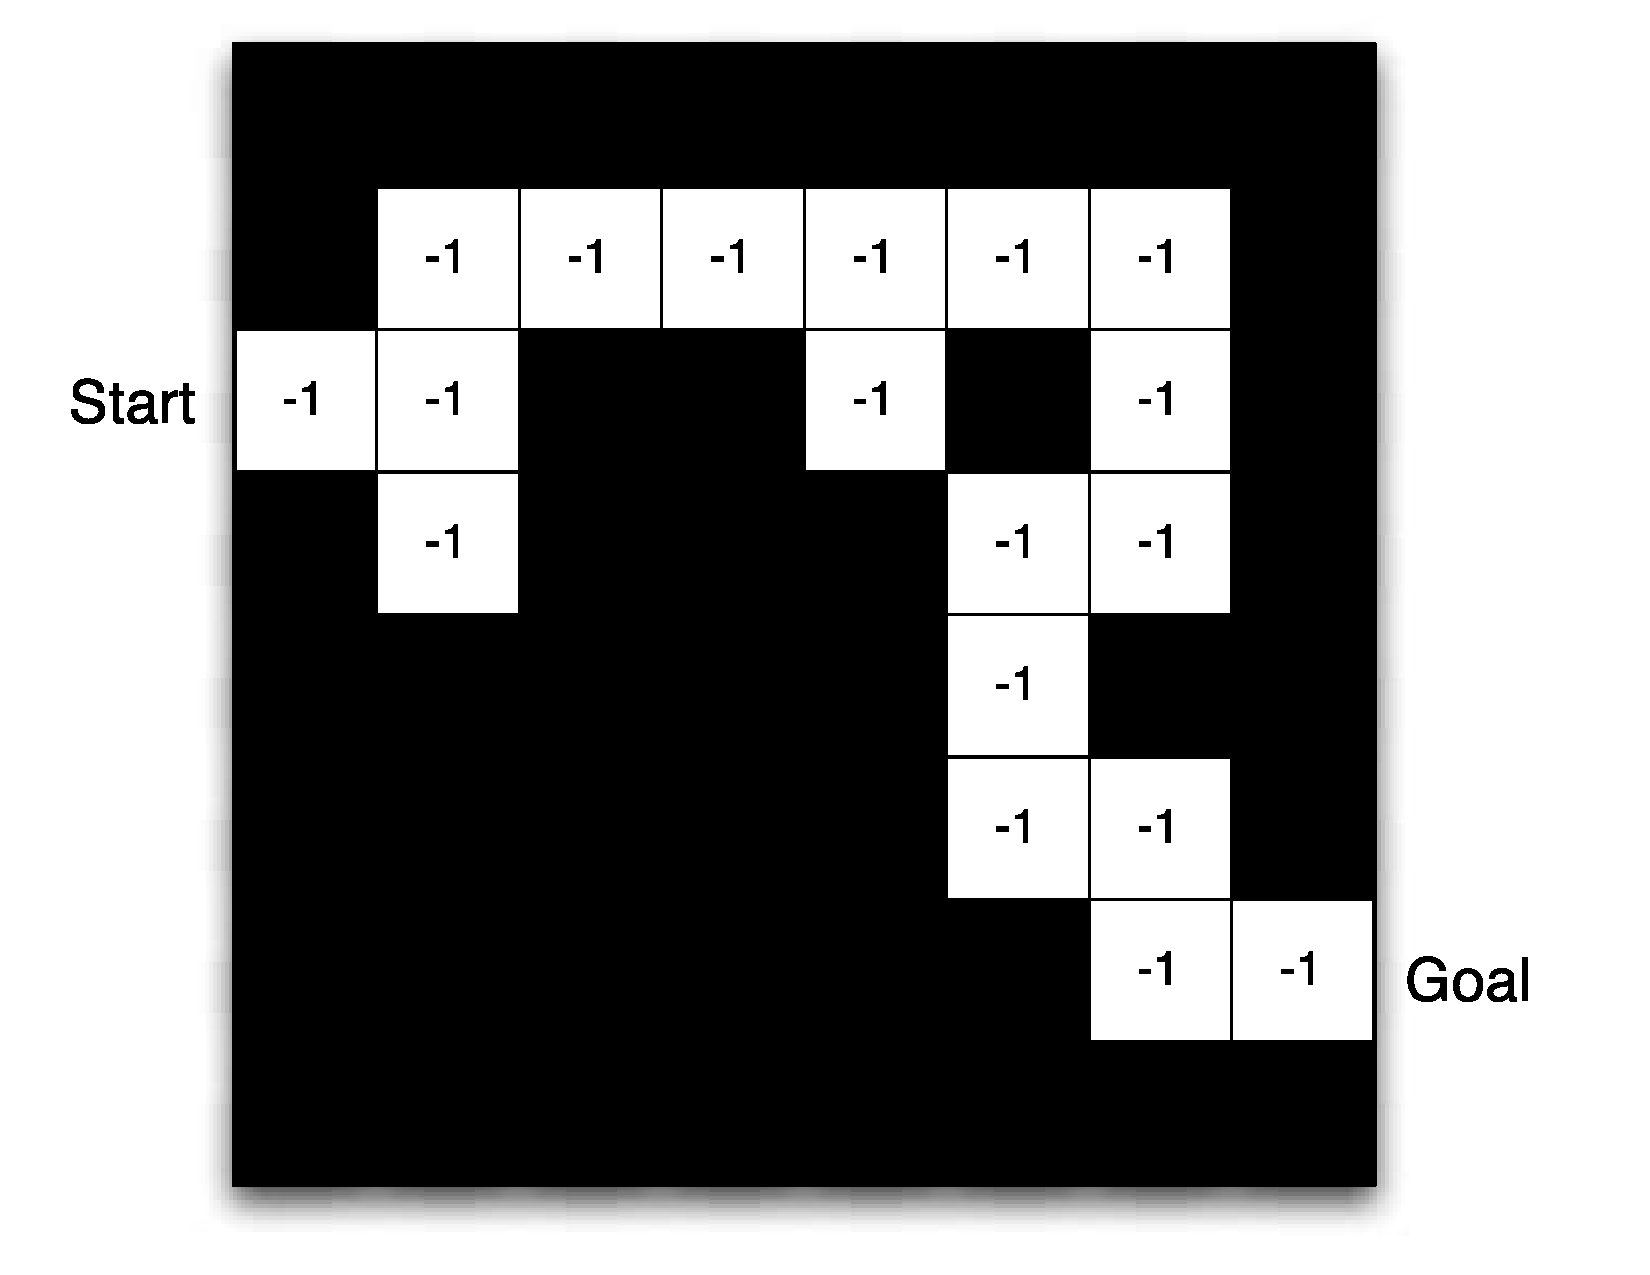
\includegraphics[width=0.5\textwidth]{img/maze_model.pdf}
\end{figure}
\begin{itemize}
\item Grid layout represent transition model $\mathcal{P}_{ss'}^a$
\item Numbers represent immediate reward $R_s^a$ from each state $s$ (same for all a)
\end{itemize}
\end{frame}
\egroup
\bgroup
\begin{frame}{RL taxonomy}
\begin{figure}
\centering
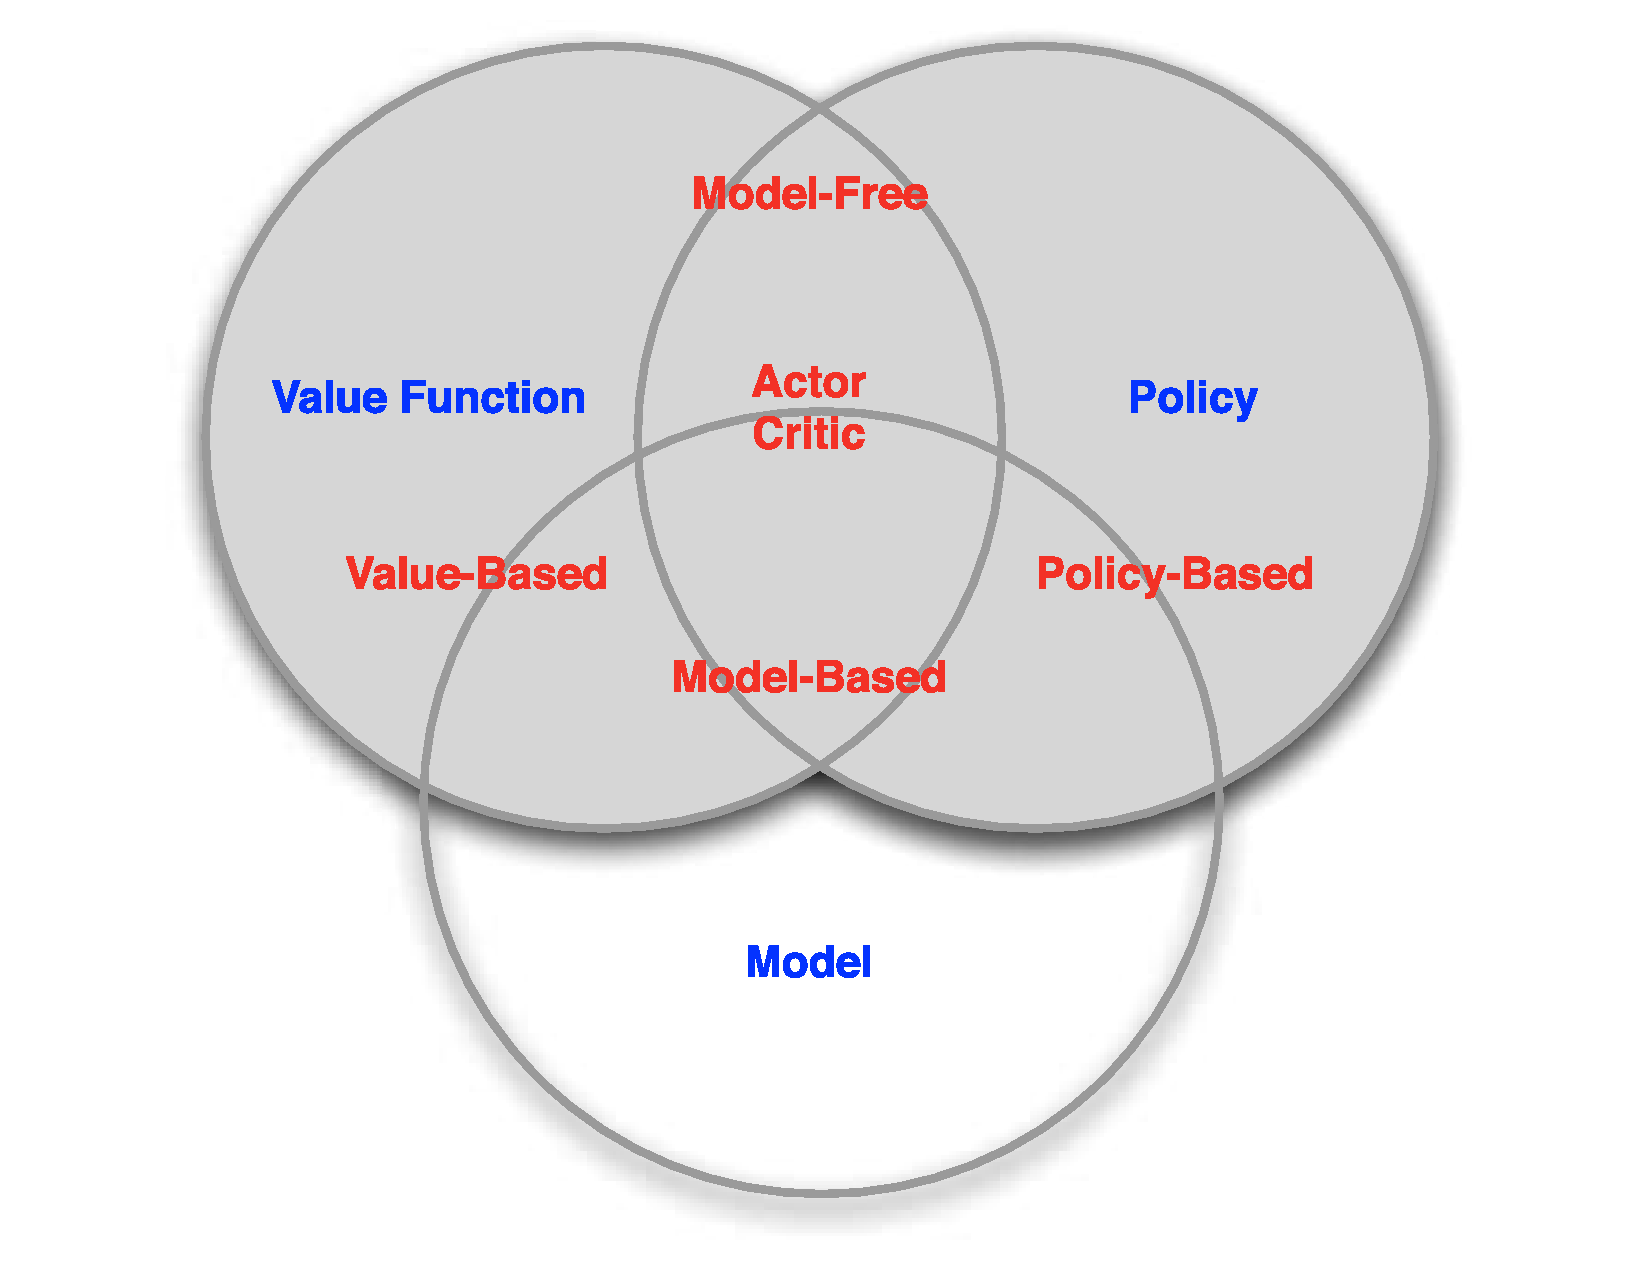
\includegraphics[width=0.65\textwidth]{img/rl_taxonomy.pdf}
\end{figure}
\end{frame}
\end{frame}
\egroup

\section{Model-free prediction}
\bgroup
\begin{frame}{Model-Free prediction}
\begin{itemize}
\item \highlight{Model-free prediction}
\begin{itemize}
\item estimate the value function given a policy in a non-observable environment
\begin{itemize}
\item Monte-Carlo Learning
\item Temporal-Difference Learning
\end{itemize}
\end{itemize}
\end{itemize}
\end{frame}
\egroup
\bgroup
\begin{frame}{Monte-Carlo reinforcement learning}
\begin{itemize}
\item MC methods learn directly from episodes of experience
\item MC is \emph{model-free}: no explicit knowledge of environment mechanisms
\item MC learns from complete episodes
\begin{itemize}
\item Caveat: can only apply to \emph{episodic} environments (all episodes must terminate).
\end{itemize}
\item MC uses the simpliest possible idea: value = mean return
\end{itemize}
\end{frame}
\egroup
\bgroup
\begin{frame}{Monte-Carlo Policy Evaluation}
\begin{itemize}
\item Goal: learn $v_{\pi}$ from episodes of experience under policy $\pi$
\begin{equation*}
S_1, A_1, R_2, \ldots, S_k \sim \pi
\end{equation*}
\item Recall that the \emph{return} is the total discounted reward:
\begin{equation*}
G_t = R_{t+1} + \gamma R_{t+2}+\ldots+\gamma^{T-1}R_T
\end{equation*}
\item Recall that the value function is the expected return:
\begin{equation*}
v_{\pi}(s) = \mathbb{E}_{\pi}[G_t | S_t = s]
\end{equation*}
\item Monte-Carlo policy evaluation uses \emph{empirical mean} return instead of \emph{expected} return
\end{itemize}
\end{frame}
\egroup
\bgroup
\begin{frame}{Every-Visit Monte-Carlo Policy Evaluation}
\begin{itemize}
\item To evaluate state $s$
\item Every time-step $t$ that state $s$ is visited in an episode,
\item Increment counter $N(s) \leftarrow N(s) + 1$
\item Increment total return $S(s) \leftarrow S(s) + Gt$
\item Value is estimated by mean return $V(s) = S(s)/N(s)$
\item By law of large numbers, $V(s) \rightarrow v_{\pi}(s)$ as $N(s) \rightarrow \infty$
\end{itemize}
\end{frame}
\egroup
\bgroup
\begin{frame}{Incremental Monte-Carlo Updates}
\begin{itemize}
\item Update $V(s)$ incrementally after episode $S_1, A_1, R_2, ..., S_T$
\item Compute return $G_t$
\item For each state $S_t$ with return $G_t$
\begin{align*}
&N(S_t) \leftarrow N(S_t) + 1 \\
&V(S_t) \leftarrow V(S_t) + \frac{1}{N(S_t)}(G_t − V(S_t))
\end{align*}
\item Usually a running mean is employed, i.e. forget old episodes
\begin{equation*}
V(S_t) \leftarrow V(S_t) + \alpha(G_t − V(S_t))
\end{equation*}
\end{itemize}
\end{frame}
\egroup
\bgroup
\begin{frame}{Blackjack Example}
\begin{minipage}{0.7\textwidth}
\begin{itemize}
\item States (200 of them):
\begin{itemize}
\item Current sum (12-21)
\item Dealer's showing card (ace-10)
\item Do I have a useable ace? (yes-no)
\end{itemize}
%
\item Action \highlight{stick}: Stop receiving cards (and terminate)
\item Action \highlight{twist}: Take another card (no replacement)
\item Reward for \highlight{stick}:
\begin{itemize}
\item +1 if sum of cards $>$ sum of dealer cards
\item 0 if sum of cards $=$ sum of dealer cards
\item -1 if sum of cards $<$ sum of dealer cards
\end{itemize}
%
\item Reward for \highlight{twist}:
\begin{itemize}
\item -1 if sum of cards $>$ 21 (and terminate)
\item 0 otherwise
\end{itemize}
%
\item Transitions: automatically \highlight{twist} if sum of cards $<$ 12
\end{itemize}
\end{minipage}
\begin{minipage}{0.25\textwidth}
\begin{figure}
\centering
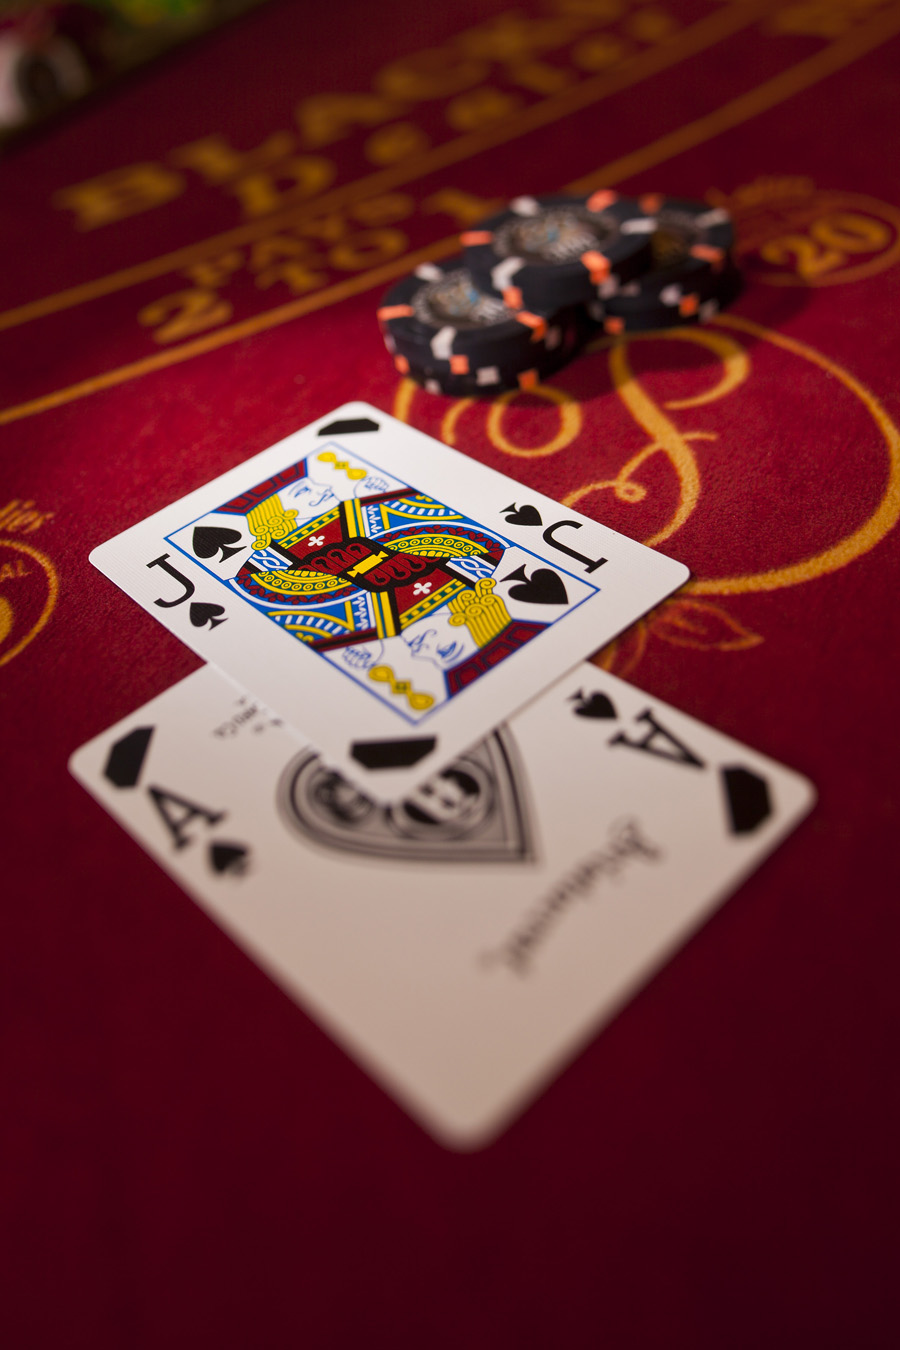
\includegraphics[width=\textwidth]{img/blackjack.jpg}
\end{figure}
\end{minipage}

\end{frame}
\egroup
\bgroup
\begin{frame}{Blackjack Value Function after Monte-Carlo Learning}
\begin{figure}
\centering
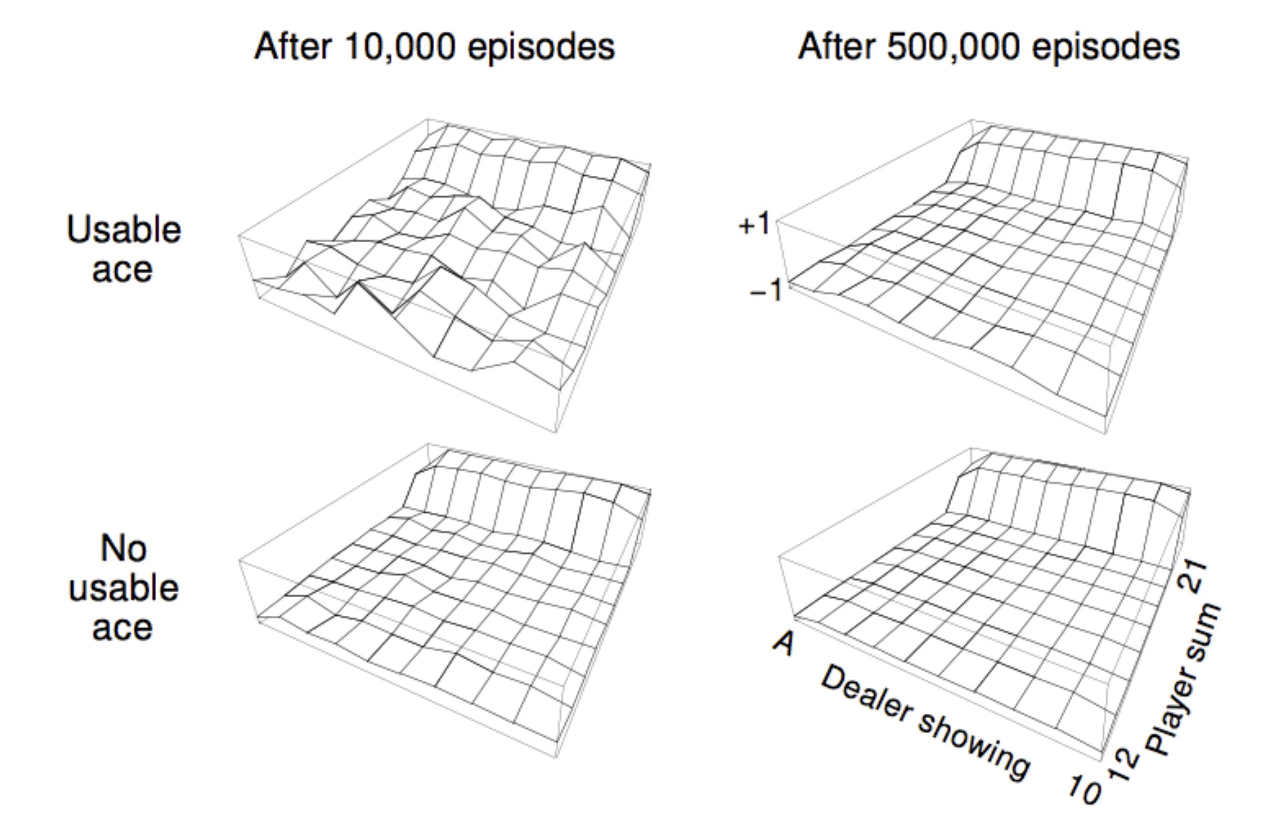
\includegraphics[width=0.657\textwidth]{img/blackjack_value.pdf}
\end{figure}
Policy: \highlight{stick} if sum of cards $\leq$20, otherwise \highlight{twist}
\end{frame}
\egroup
\bgroup
\begin{frame}{MC and TD}
\begin{itemize}
\item Goal: learn $v_{\pi}$ online from experience under policy $\pi$
\item Incremental every-visit Monte-Carlo
\begin{itemize}
\item Update value $V(S_t)$ toward actual return \highlight{$G_t$}
\begin{equation*}
V(S_t) \leftarrow V(S_t) +\alpha (\highlight{G_t} − V(S_t))
\end{equation*}
\end{itemize}
%
\item Simplest temporal-difference learning algorithm: TD(0)
\begin{itemize}
\item Update value $V(S_t)$ toward estimated return \highlight{$R_{t+1} + \gamma V(S_{t+1})$}
\begin{equation*}
V(S_t) \leftarrow V(S_t) + \alpha (\highlight{R_{t+1} + \gamma V(S_{t+1})} − V(S_t))
\end{equation*}
\item $R_{t+1} + \gamma V(S_{t+1})$ is called the TD target
\item $\delta_t = R_{t+1} + \gamma V(S_{t+1}) − V(S_t)$ is called the TD error
\end{itemize}
\end{itemize}
\end{frame}
\egroup
\bgroup
\begin{frame}{Driving home example: MC vs. TD}
\begin{figure}
\centering
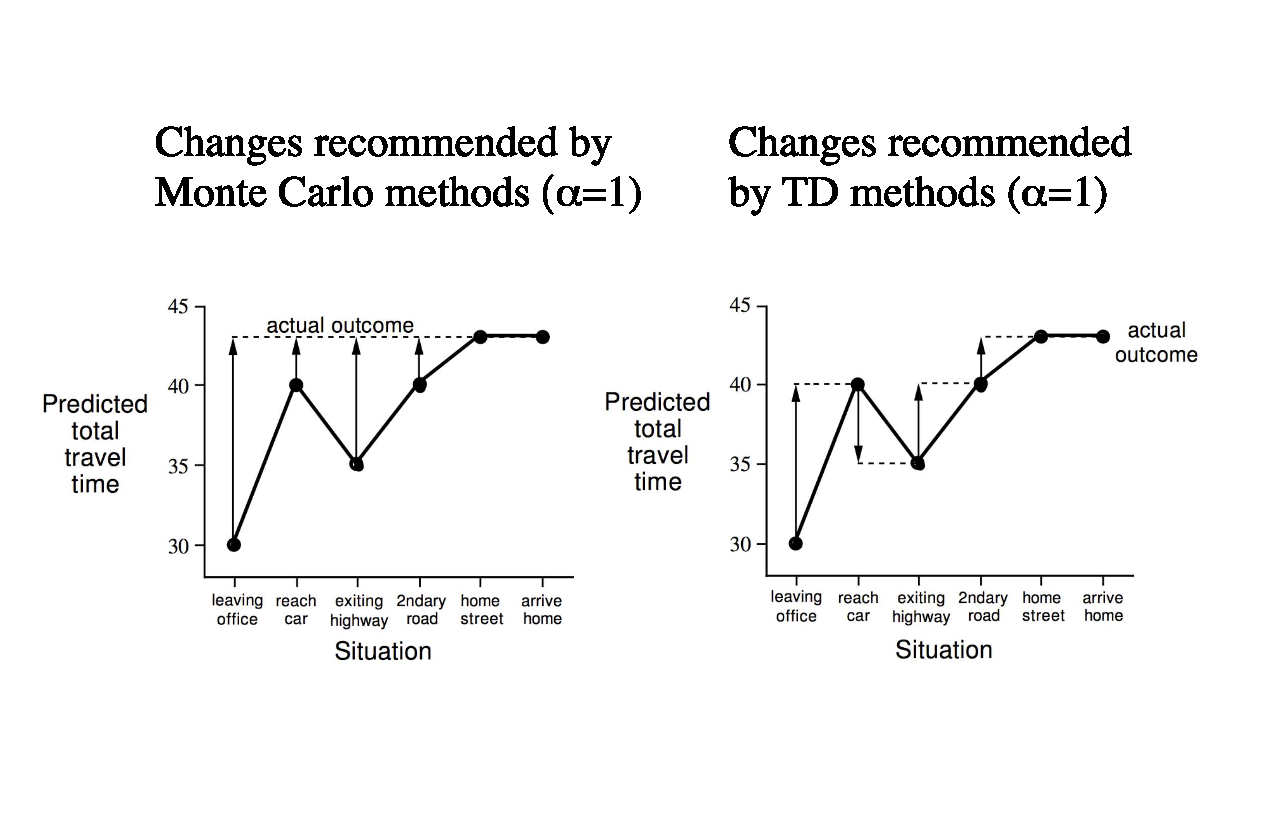
\includegraphics[width=0.9\textwidth]{img/go_home_example.pdf}
\end{figure}
\end{frame}
\egroup
\bgroup
\begin{frame}{Advantages and disadvantages of MC vs. TD}
\begin{itemize}
\item TD can learn \emph{before} knowing the final outcome
\begin{itemize}
\item TD can learn online after every step
\item MC must wait until end of episode before return is known
\end{itemize}
\item TD can learn without the final outcome
\begin{itemize}
\item TD can learn from incomplete sequences
\item MC can only learn from complete sequences
\item TD works in continuing (non-terminating) environments
\item MC only works for episodic (terminating) environments
\end{itemize}
\end{itemize}
\end{frame}
\egroup
\bgroup
\begin{frame}{Bias/variance trade-off}
\begin{itemize}
\item Return $G_t=R_{t+1}+R_{t+2}+\ldots+\gamma^{T-1}R_T$ is \emph{unbiased} estimate of $v_{\pi}(S_t)$
\item True TD target $R_{t+1}+v_{\pi}(S_{t+1})$ is unbiased estimate of $v_{\pi}(S_t)$
\item TD target $R_{t+1}+v(S_{t+1})$ is biased estimate of $v_{\pi}(S_t)$
\item TD target is much lower variance than the return:
\begin{itemize}
\item Return depends on many random actions, transitions, rewards
\item TD target depends on one random action, transition, reward
\end{itemize}
\end{itemize}
\end{frame}
\egroup

\section{Model-free control}
\bgroup
\begin{frame}{Model-Free control}
\begin{itemize}
\item \highlight{Model-free prediction}
\begin{itemize}
\item estimate the value function given a policy in a non-observable environment
\begin{itemize}
\item Monte-Carlo Learning
\item Temporal-Difference Learning
\end{itemize}
\end{itemize}
\item \highlight{Model-free control}
\begin{itemize}
\item find a good policy in a non-observable environment
\begin{itemize}
\item On-Policy Monte-Carlo Control
\item On-Policy Temporal-Difference Learning
\item Off-Policy Learning
\end{itemize}
\end{itemize}
\end{itemize}
\end{frame}
\egroup
\bgroup
\begin{frame}{How to improve a policy}
\begin{itemize}
\item Given a policy $\pi$
\item Evaluate the policy $\pi$
\begin{align*}
v_{\pi}(s) &= \mathbb{E}[R_{t+1} + \gamma R_{t+2} + \ldots|S_t = s]\\
q_{\pi}(s, a) &= \mathbb{E}[R_{t+1} + \gamma R_{t+2} + \ldots|S_t = s, A_t = a]\\
\end{align*}
\item Improve the policy by acting greedily with respect to $v_{\pi}$
\begin{align*}
\pi^{\prime} &=\text{greedy}(v_{\pi})\\
\pi^{\prime} &=\text{greedy}(q_{\pi})
\end{align*}
\item In general, need more iterations of improvement / evaluation
\item In model-free contexts, action-value function $Q(s, a)$ is our only option
\end{itemize}
\end{frame}
\egroup
\bgroup
\begin{frame}{Example of greedy action selection}
\begin{minipage}{0.4\textwidth}
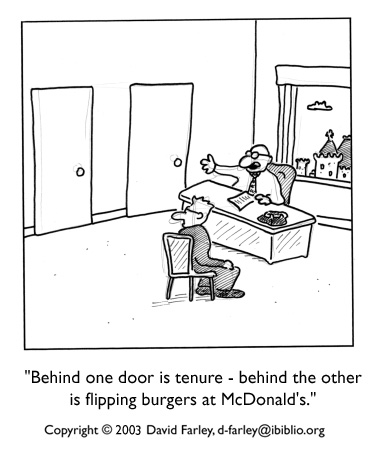
\includegraphics[width=\textwidth]{img/doors.jpg}
\end{minipage}
\begin{minipage}{0.55\textwidth}
\begin{itemize}
\item There are two doors in front of you.
\item You open the left door and get reward 0\\
\highlight{V(left) = 0}
\item You open the right door and get reward +1\\
\highlight{V(right) = +1}
\item You open the right door and get reward +3\\
\highlight{V(right) = +2}
\item You open the right door and get reward +2\\
\highlight{V(right) = +2}
\begin{equation*}
\vdots
\end{equation*}
\item Are you sure you've chosen the best door?
\end{itemize}
\end{minipage}
\end{frame}
\egroup
\bgroup
\begin{frame}{$\epsilon$-greedy exploration}
\begin{itemize}
\item Simplest idea for ensuring continual exploration
\item All $m$ actions are tried with non-zero probability
\item With probability 1 − $\epsilon$ choose the greedy action 
\item With probability $\epsilon$ choose an action at random
\end{itemize}
\begin{equation*}
\pi(a|s) = \begin{cases}
    \epsilon / m + 1 - \epsilon,& \text{if } a^{\ast} = \argmax_{a \in \mathcal{A}} Q(s,a)\\
    \epsilon / m,              & \text{otherwise}
\end{cases}
\end{equation*}
\end{frame}
\egroup
\bgroup
\begin{frame}{On and off policy learning}
\begin{itemize}
\item \highlight{On-policy learning} 
\begin{itemize}
\item ``Learn on the job''
\item Learn about policy $\pi$ from experience sampled from $\pi$
\end{itemize}
\item \highlight{Off-policy learning}
\begin{itemize}
\item ``Look over someone’s shoulder''
\item Learn about policy $\pi$ from experience sampled from $\mu$
\end{itemize}
\end{itemize}
\end{frame}
\egroup
\bgroup
\begin{frame}{Monte-Carlo policy iteration}
\begin{figure}
\centering
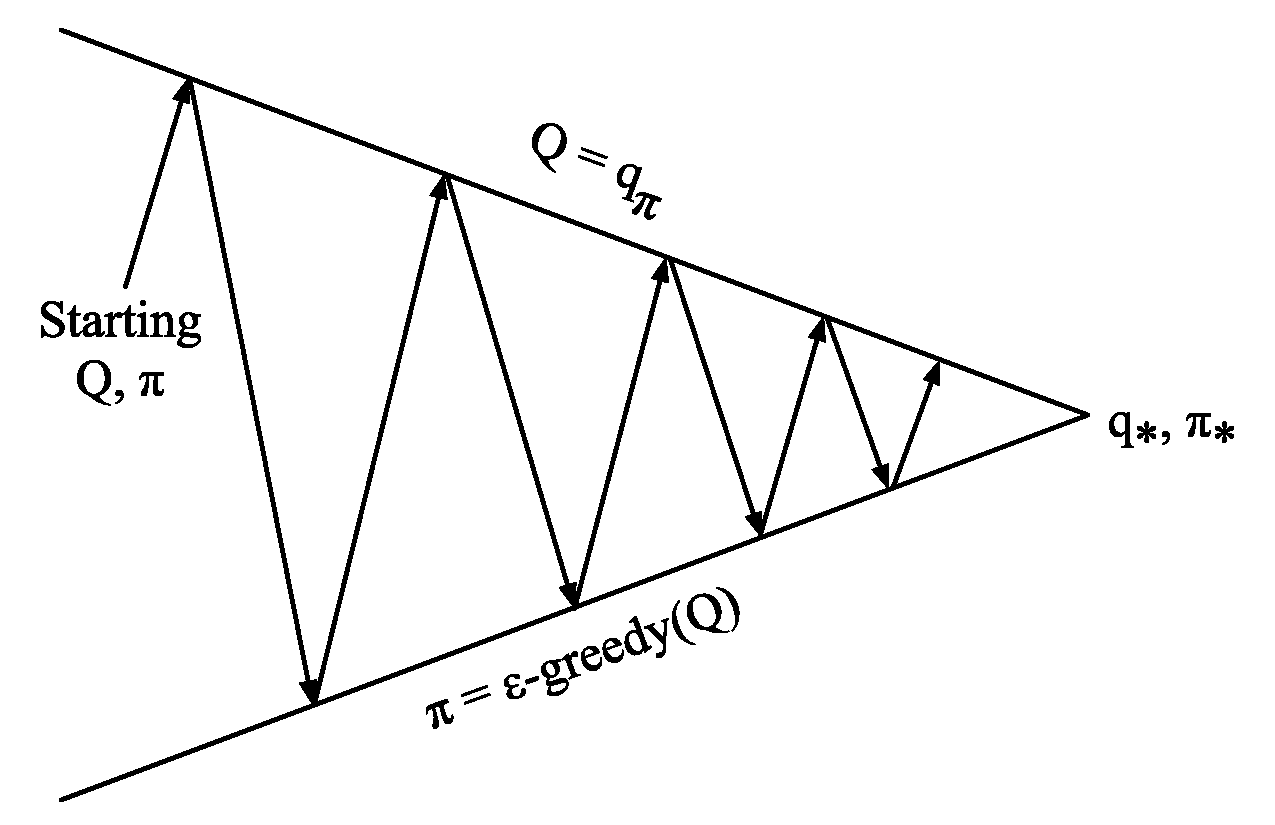
\includegraphics[width=0.5\textwidth]{img/mc_policy_iteration.pdf}
\end{figure}
\highlight{Policy evaluation} Monte-Carlo policy evaluation, $Q=q_{\pi}$\\
\highlight{Policy improvement} \highlight{$\epsilon$}-greedy policy improvement
\end{frame}
\egroup
\bgroup
\begin{frame}{Monte-Carlo control}
\begin{figure}
\centering
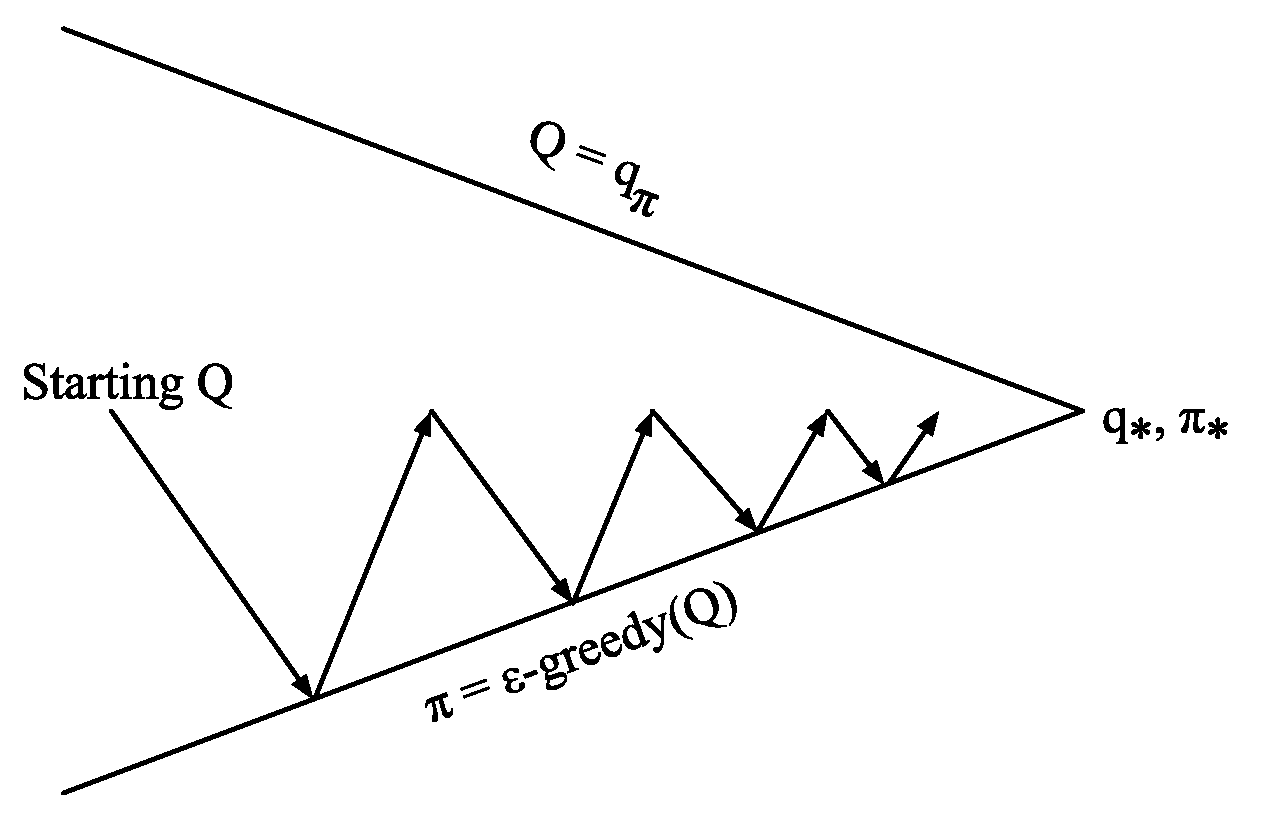
\includegraphics[width=0.5\textwidth]{img/mc_control.pdf}
\end{figure}
\highlight{Every episode:}\\
\highlight{Policy evaluation} Monte-Carlo policy evaluation, $Q=q_{\pi}$\\
\highlight{Policy improvement} $\epsilon$-greedy policy improvement
\end{frame}
\egroup
\bgroup
\begin{frame}{Back to the blackjack example}
\centering
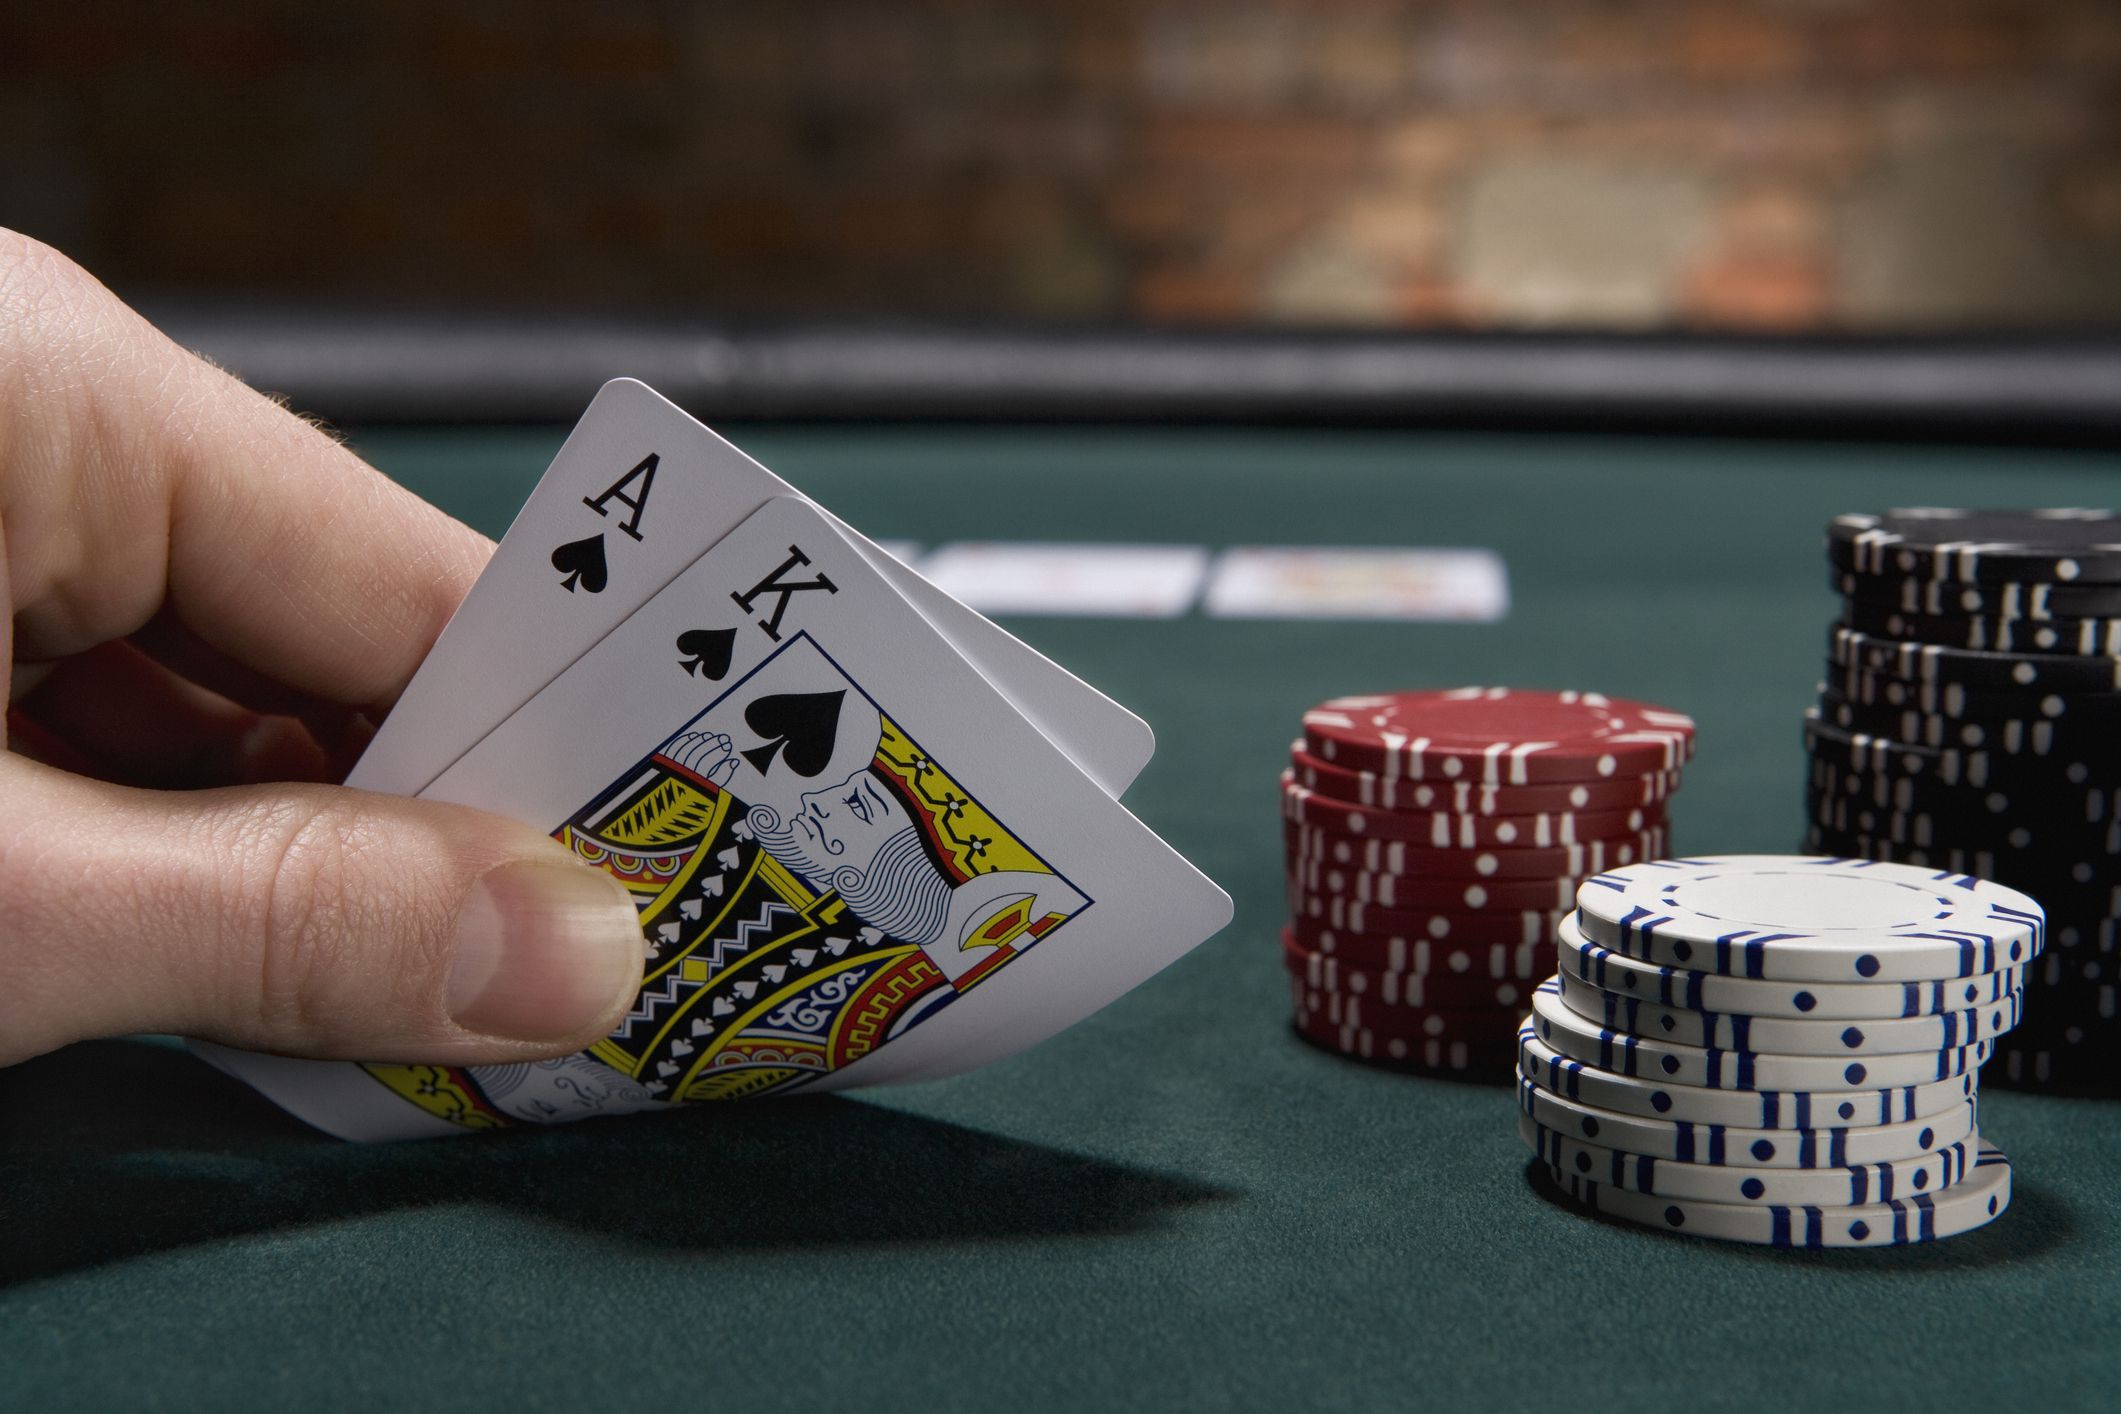
\includegraphics[width=0.75\textwidth]{img/blackjack2.jpg}
\end{frame}
\egroup
\bgroup
\begin{frame}{Monte-Carlo control in blackjack}
\begin{figure}
\centering
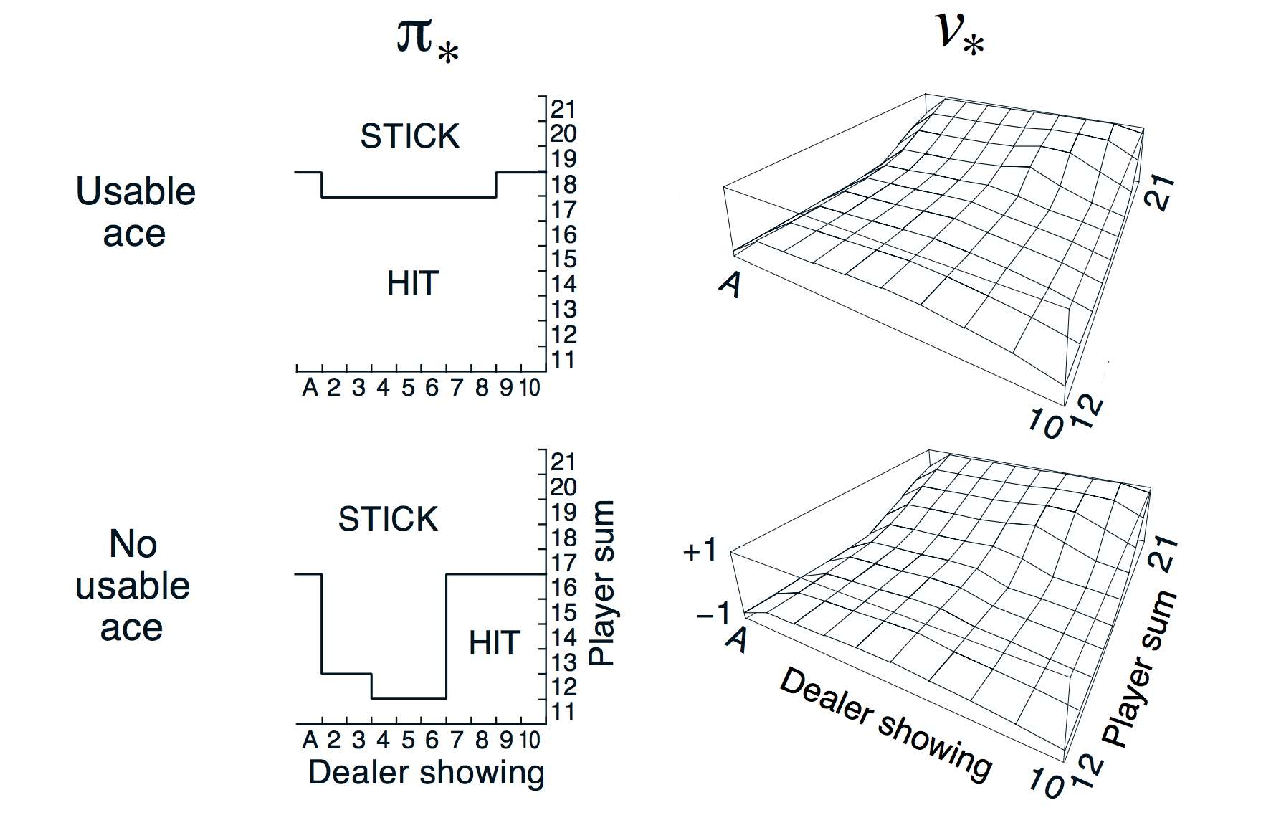
\includegraphics[width=0.7\textwidth]{img/blackjack_mc_control.pdf}
\end{figure}
\end{frame}
\egroup
\bgroup
\begin{frame}{MC vs TD control}
\begin{itemize}
\item Temporal-difference (TD) learning has several advantages over Monte-Carlo (MC)
\begin{itemize}
\item Lower variance
\item Online
\item Incomplete sequences
\end{itemize}
\item Natural idea: use TD instead of MC in our control loop
\begin{itemize}
\item Apply TD to $Q(S, A)$
\item Use $\epsilon$-greedy policy improvement
\item Update every time-step
\end{itemize}
\end{itemize}
\end{frame}
\egroup
\bgroup
\begin{frame}{Updating action-value functions with SARSA}
\begin{figure}
\centering
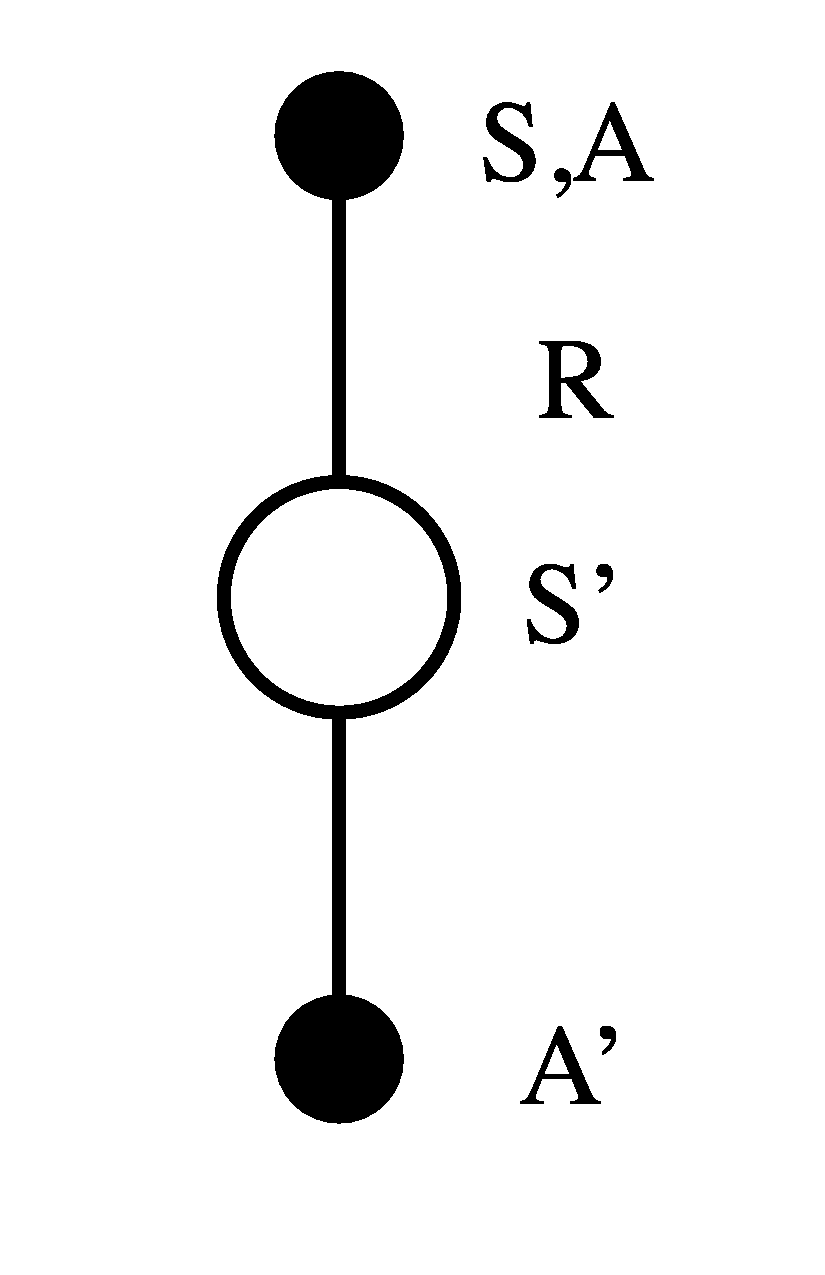
\includegraphics[width=0.2\textwidth]{img/sarsa.pdf}
\end{figure}
\begin{equation*}
Q(S,A) \leftarrow Q(S,A) + \alpha (R + \gamma Q(S^{\prime}, A^{\prime}) - Q(S,A))
\end{equation*}
\end{frame}
\egroup
\bgroup
\begin{frame}{On-policy control with SARSA}
\begin{figure}
\centering
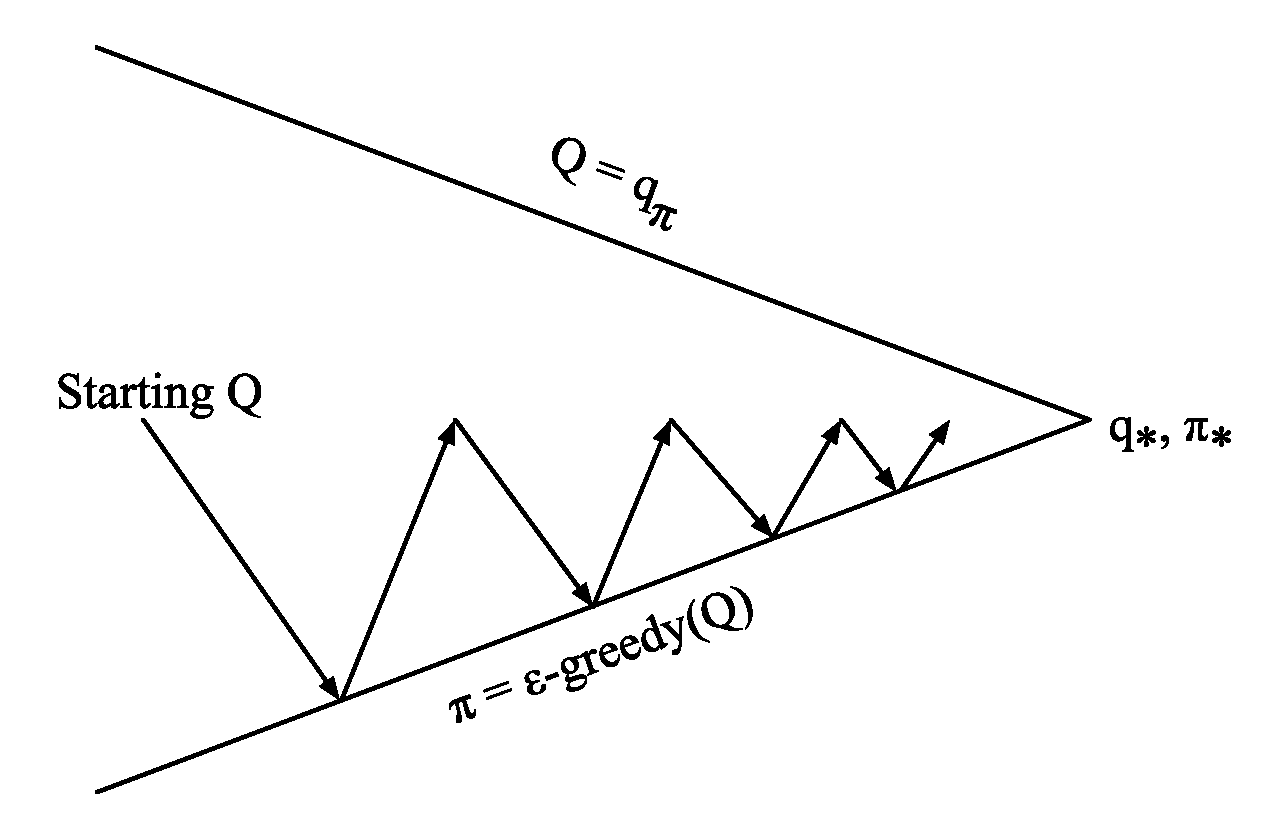
\includegraphics[width=0.5\textwidth]{img/sarsa_control.pdf}
\end{figure}
Every \highlight{time-step}:\\
\highlight{Policy evaluation} with \highlight{Sarsa}, $Q\approx q_{\pi}$\\
\highlight{Policy improvement} with $\epsilon$-greedy policy improvement.
\end{frame}
\egroup
\bgroup
\begin{frame}{SARSA algorithm for on-policy control}
\begin{algorithmic}
\STATE Initialize $Q(s,a), \forall s \in S, a \in \mathcal{A}(s)$, arbitrarily, and $Q(terminal-state, \dot)=0$
\FOR{each episode}
\STATE Intialise $S$
\STATE Choose $A$ from $S$ using policy derived from $Q$ (e.g., $\epsilon$-greedy)
\FOR {each step of episode}
\STATE Take action $A$, observe $R$, $S^{\prime}$
\STATE Choose $A^{\prime}$ from $S^{\prime}$ using policy derived from $Q$ (e.g., $\epsilon$-greedy)
\STATE $Q(S,A) \leftarrow Q(S,A) + \alpha (R + \gamma Q(S^{\prime}, A^{\prime}) - Q(S,A))$
\STATE $S \leftarrow S^{\prime}; A \leftarrow A^{\prime}$
\ENDFOR
\ENDFOR
\end{algorithmic}
\end{frame}
\egroup
\bgroup
\begin{frame}{Windy gridworld example}
\begin{figure}
\centering
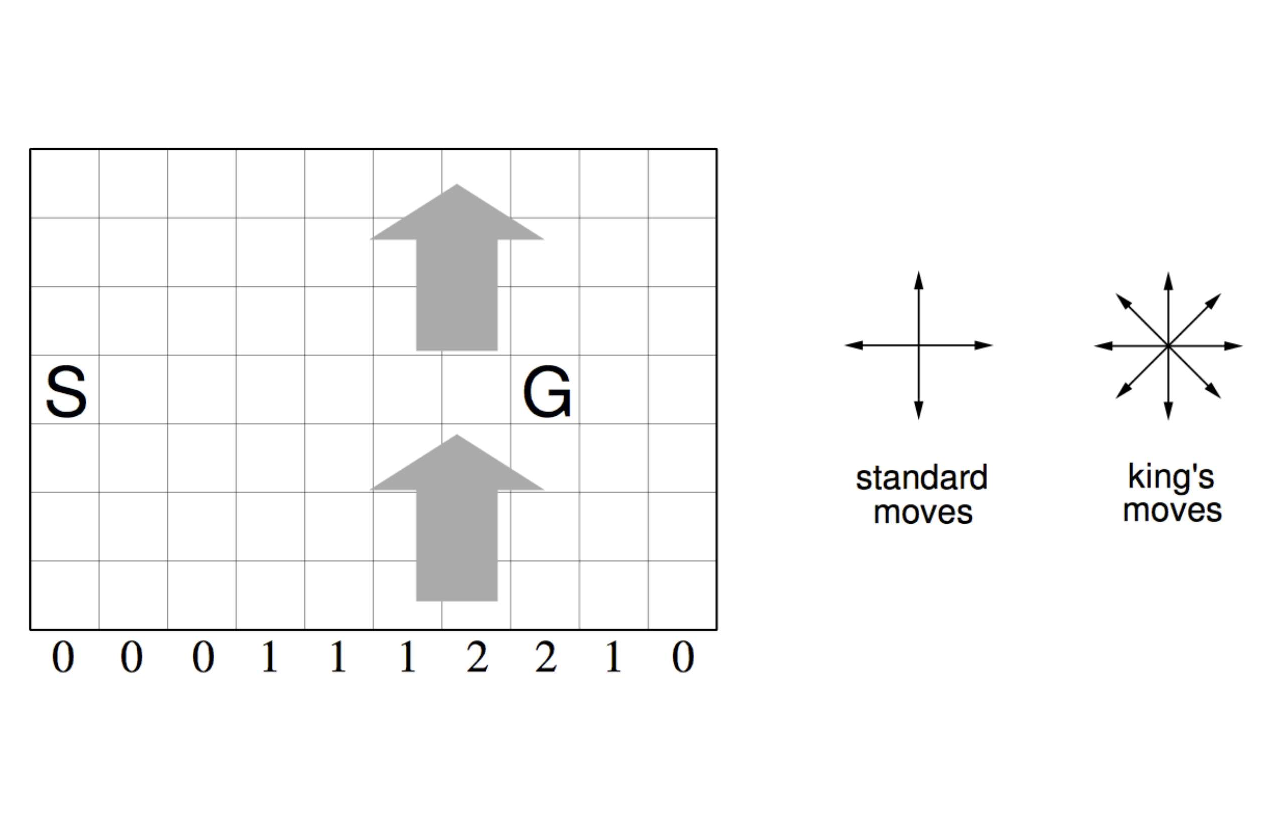
\includegraphics[width=0.7\textwidth]{img/windy_gridworld.pdf}
\end{figure}
\begin{itemize}
\item Reward = -1 per time step until reaching goal
\item Undiscounted
\end{itemize}
\end{frame}
\egroup
\bgroup
\begin{frame}{SARSA on the Windy Gridworld}
\begin{figure}
\centering
\hspace{-1cm}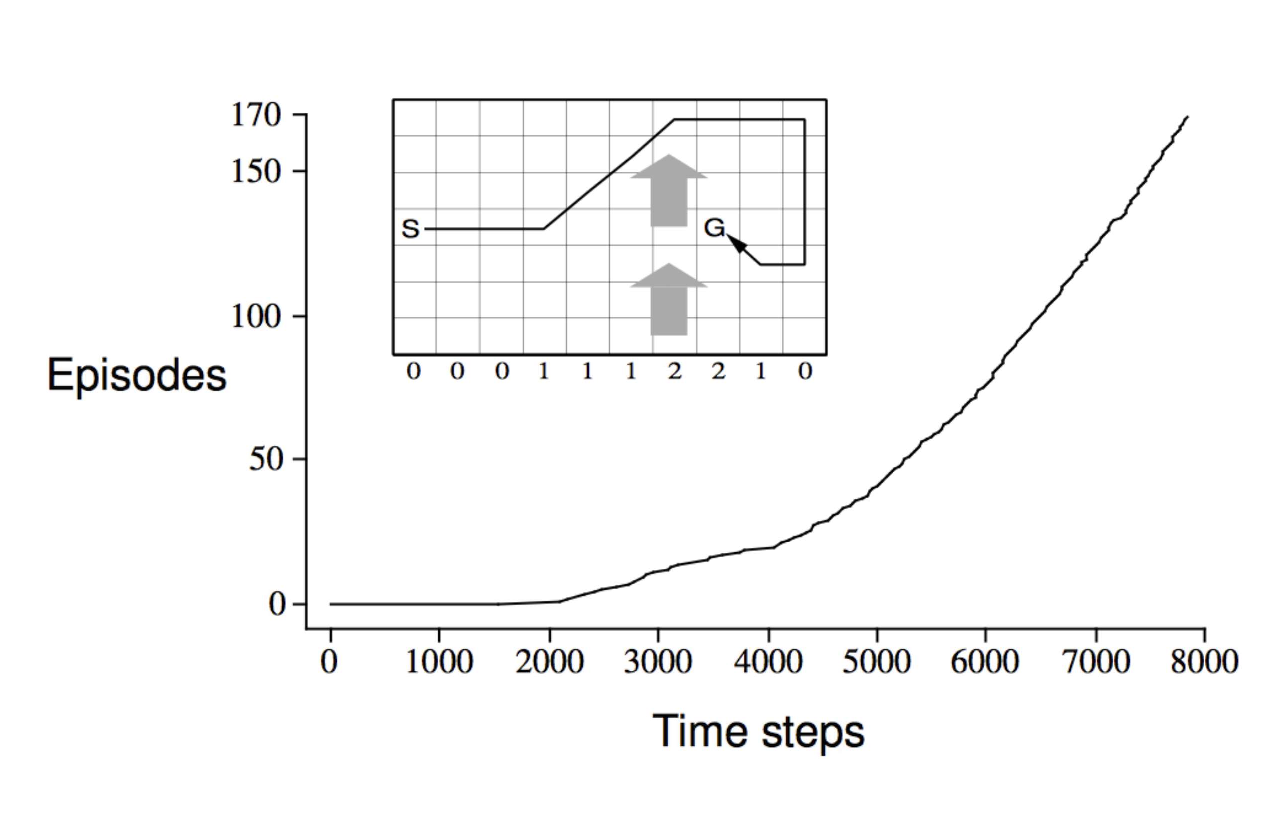
\includegraphics[width=0.8\textwidth]{img/sarsa_windy_gridworld.pdf}
\end{figure}
\end{frame}
\egroup
\bgroup
\begin{frame}{Off-policy learning}
\begin{itemize}
\item Evaluate target policy $\pi(a,s)$ to compute $v_{\pi}(s)$ or $q_{\pi}(s, a)$
\item While following behaviour policy $\mu(a|s)$
\begin{equation*}
\{S_1, A_1, R_2, \ldots, S_T\} \sim \mu
\end{equation*}
\item Why is this important?
\item Learn from observing humans or other agents
\item Re-use experience generated from old policies $\pi_1, \pi_2, \ldots, \pi_{t-1}$
\item Learn about \emph{optimal} policy while following \emph{exploratory} policy
\item Learn about \emph{multiple} policies while following \emph{one} policy
\end{itemize}
\end{frame}
\egroup
\documentclass[aspectratio=169]{beamer}
%
% Choose how your presentation looks.
%
% For more themes, color themes and font themes, see:
% http://deic.uab.es/~iblanes/beamer_gallery/index_by_theme.html
%
\mode<presentation>
{
  \usetheme{metropolis}      % or try Darmstadt, Madrid, Warsaw, ...
  \usecolortheme{metropolis-imagelab} % or try albatross, beaver, crane, ...
  \usefonttheme{structurebold}  % or try serif, structurebold, ...
  \setbeamercolor{background canvas}{bg=white}
  \setbeamertemplate{navigation symbols}{}
  \setbeamertemplate{bibliography item}{\insertbiblabel}
  %\setbeamertemplate{caption}[numbered]
} 
\usepackage[english]{babel}
\usepackage[utf8x]{inputenc}
\usepackage{algorithmic}
\usepackage{hyperref}
\usepackage{listings}             % Include the listings-package
\hypersetup{
    colorlinks = true,
    linkcolor = {mImagelabRed},
    urlcolor = {mImagelabRed}
}
\usepackage{animate}

\DeclareMathOperator*{\argmin}{arg\,min}

\title[Q-Learning]{Q-Learning}
\subtitle{Pattern Recognition and Machine Learning - 2017}
\institute{University of Modena and Reggio Emilia}
\author{Andrea Palazzi, Davide Abati}
\date{\today}

\def\thisframelogos{}

\newcommand{\framelogo}[1]{\def\thisframelogos{#1}}

\begin{document}

\framelogo{logo_unimore_white.png}

\bgroup
\renewcommand{\insertframenumber}{}
\begin{frame}[noframenumbering]
  \titlepage
\end{frame}
\egroup
\bgroup
\begin{frame}{Problem setting}
\begin{minipage}{0.5\textwidth}
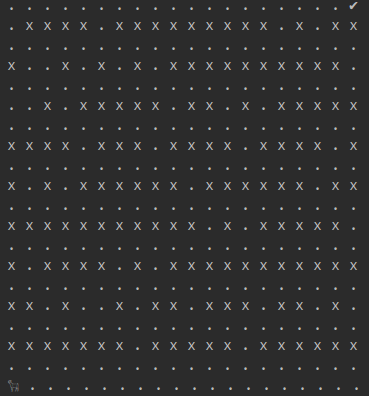
\includegraphics[width=0.9\textwidth]{img/env.png}
\end{minipage}
\begin{minipage}{0.45\textwidth}
We have an agent stuck in a maze.
\begin{itemize}
\item state is (x,y) position
\item reward is -1 for each time step
\item when the exit of the labirinth is reached, the episode terminates
\item allowed actions are N,S,W,E
\end{itemize}
Guide him out with reinforcement learning!
\end{minipage}
\end{frame}
\egroup
\bgroup
\begin{frame}{Q-learning algorithm for off-policy control}
\begin{algorithmic}
\STATE Initialize $Q(s,a), \forall s \in S, a \in \mathcal{A}(s)$, arbitrarily, and $Q(terminal-state, \dot)=0$
\FOR{each episode}
\STATE Intialise $S$
\FOR {each step of episode}
\STATE Choose $A$ from $S$ using policy derived from $Q$ (e.g., $\epsilon$-greedy)
\STATE Take action $A$, observe $R$, $S^{\prime}$
\STATE $Q(S,A) \leftarrow Q(S,A) + \alpha (R + \gamma \max_{a^{\prime}}Q(S^{\prime}, a^{\prime}) - Q(S,A))$
\STATE $S \leftarrow S^{\prime}$
\ENDFOR
\ENDFOR
\end{algorithmic}
\end{frame}
\egroup
\bgroup
\begin{frame}{SARSA algorithm for on-policy control}
\begin{algorithmic}
\STATE Initialize $Q(s,a), \forall s \in S, a \in \mathcal{A}(s)$, arbitrarily, and $Q(terminal-state, \dot)=0$
\FOR{each episode}
\STATE Intialise $S$
\STATE Choose $A$ from $S$ using policy derived from $Q$ (e.g., $\epsilon$-greedy)
\FOR {each step of episode}
\STATE Take action $A$, observe $R$, $S^{\prime}$
\STATE Choose $A^{\prime}$ from $S^{\prime}$ using policy derived from $Q$ (e.g., $\epsilon$-greedy)
\STATE $Q(S,A) \leftarrow Q(S,A) + \alpha (R + \gamma Q(S^{\prime}, A^{\prime}) - Q(S,A))$
\STATE $S \leftarrow S^{\prime}; A \leftarrow A^{\prime}$
\ENDFOR
\ENDFOR
\end{algorithmic}
\end{frame}
\egroup
\bgroup
\begin{frame}{More fun with gym!}
If you are curious about RL, try \href{https://github.com/openai/gym}{gym}:
\begin{center}
pip install gym
\end{center}
\centering
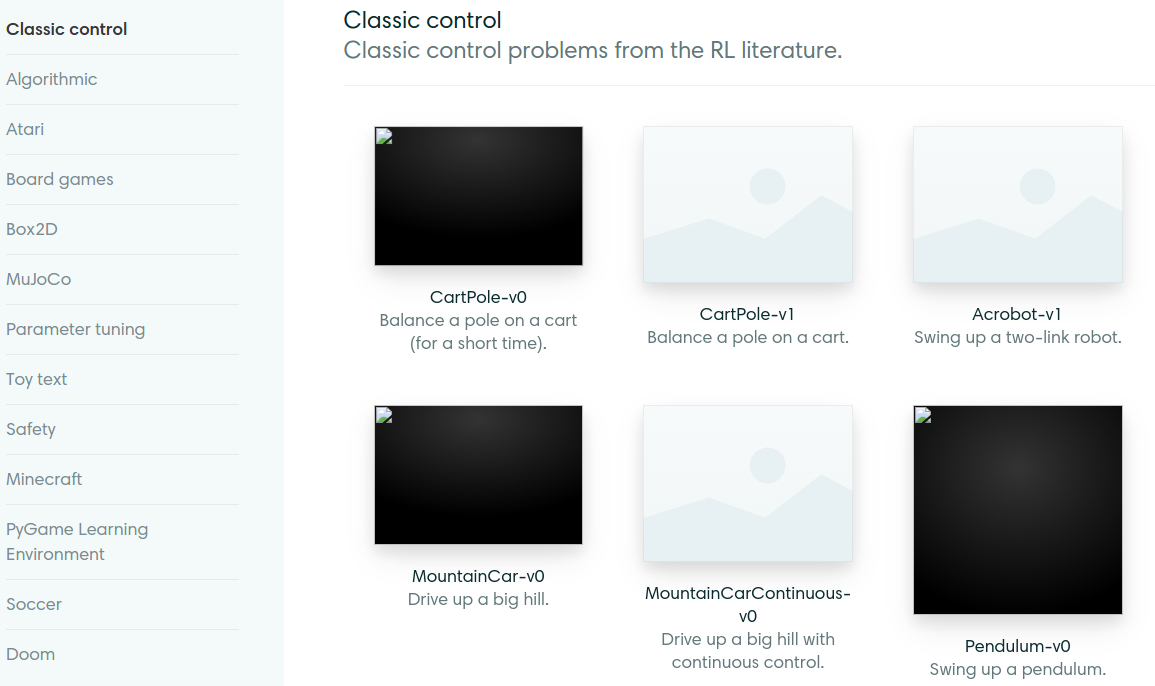
\includegraphics[width=0.5\textwidth]{img/gym.png}
\end{frame}
\egroup

\end{document}
\bgroup
\begin{frame}{Off-policy control with Q-learning}
\begin{itemize}
\item We now allow both behaviour and target policies to \highlight{improve}
\item The target policy $\pi$ is \highlight{greedy} w.r.t. $Q(s, a)$
\begin{equation*}
\pi(S_{t+1}) = \argmax_{a^{\prime}}Q(S_{t+1}, a^{\prime})
\end{equation*}
\item The behaviour policy $\mu$ is \highlight{$\epsilon$-greedy} w.r.t. $Q(s, a)$
\item The Q-learning target then simplifies:
\begin{align*}
& R_{t+1} + \gamma Q(S_{t+1}, A^{\prime})\\
=& R_{t+1} + \gamma Q(S_{t+1}, \argmax_{a^{\prime}} Q(S_{t+1}, a^{\prime}))\\
=& R_{t+1} + \gamma \max_{a^{\prime}}Q(S_{t+1},a^{\prime})
\end{align*}
\end{itemize}
\end{frame}
\egroup
\bgroup
\begin{frame}{Q-learning algorithm for off-policy control}
\begin{algorithmic}
\STATE Initialize $Q(s,a), \forall s \in S, a \in \mathcal{A}(s)$, arbitrarily, and $Q(terminal-state, \dot)=0$
\FOR{each episode}
\STATE Intialise $S$
\FOR {each step of episode}
\STATE Choose $A$ from $S$ using policy derived from $Q$ (e.g., $\epsilon$-greedy)
\STATE Take action $A$, observe $R$, $S^{\prime}$
\STATE $Q(S,A) \leftarrow Q(S,A) + \alpha (R + \gamma \max_{a^{\prime}}Q(S^{\prime}, a^{\prime}) - Q(S,A))$
\STATE $S \leftarrow S^{\prime}$
\ENDFOR
\ENDFOR
\end{algorithmic}
\end{frame}
\egroup

\end{document}